%!TEX root = bachelor.tex
\chapter{Methodik}
\label{ch:method}
In diesem Kapitel stellen wir zwei Vorgehensweisen zur Entzerrung von Kegeloberflächen vor. 
Zunächst gehen wir auf das verwendete Kalibrierungsmuster ein, worauf hin die einzelnen Schritte der Entzerrung erläutert werden. 

Die geometrischen Eigenschaften des Kegelstumpfs $(r, R, \Delta H)$ können gemessen und somit als bekannt angenommen werden. 
Darüber hinaus nehmen wir an, dass sich das Zentrum des kleineren Kreises im links-händigen Weltkoordinatensystem an der Positon $(0,0,0)$ (siehe Abbildung \ref{fig:coneFrustum} in Kapitel \ref{s:cone}) befindet. Durch diese Einschränkung gehen jegliche absolute Größenverhältnisse verloren. Die Larven können jedoch weiterhin relativ zu einander verglichen werden. 


\section{Kalibrierungsmuster}
\label{s:calibrationPattern}
\subsection{Aufbau des Kalibrierungsmusters}
Um eine Beziehung zwischen Bildpunkten und Kegelpunkten herstellen zu können, ist ein Kalibrierungsmuster notwendig.

Die Wahl des Kalibrierungsmusters spielt dabei eine entscheidende Rolle bei der Robustheit und Präzision der Entfaltung. Es muss gewährleistet sein, dass die charakteristischen Merkmale des Musters auch bei leichten Abweichungen der Kamera vom Lot und schlechteren Beleuchtungssituationen zuverlässig erkannt werden. Das Muster muss darüber hinaus so entworfen sein, dass beim Zusammenlegen im Kegel, dessen geometrische Eigenschaften nicht verfälscht, sondern realitätsgetreu wiedergeben werden. 

Wir haben uns für ein Muster entscheiden, dass in äquidistanten Abständen $\Delta R$, beginnend mit dem kleinen Radius $r$ des Kegelstumpfs (siehe Abbildung \ref{fig:coneFrustum}) Kreislinien und in gleichen Winkelabständen $\Delta \alpha$ auf der Seitenhöhe Liniensegmente besitzt. Das zusammengelegte Muster ist in Abbildung \ref{fig:calibrationPatternTop} zu sehen, beziehungsweise das entfaltete in \ref{fig:calibrationPattern}. Die Anzahl der Kreislinien wird mit $n$ gekennzeichnet, die Anzahl sichtbarer Liniensegmente im Kegel mit $m$. Zu beachten ist, dass bedingt durch das Entfalten, in Abbildung \ref{fig:calibrationPattern}  ein Liniensegment doppelt zu sehen ist. Die schwarzen Kreise bezeichnen wir als Samples. 

Dadurch dass die Geometrie des Kegels bekannt ist, kann jedem Sample nun ein Punkt auf dem Kegel im Weltkoordinatensystem zugeordnet werden. Da ein Kegel beliebig um die $Y$-Achse rotiert werden kann, ist diese Zuordnung zunächst nicht eindeutig. Dazu nehmen wir an, dass das Liniensegment mit dem kleinsten Winkel zur $X$-Achse mit dem Kegelwinkel $\theta = 0$ korrespondiert (siehe \ref{eq:paramFrustum}).

\begin{figure}[!htb]
	\centering
	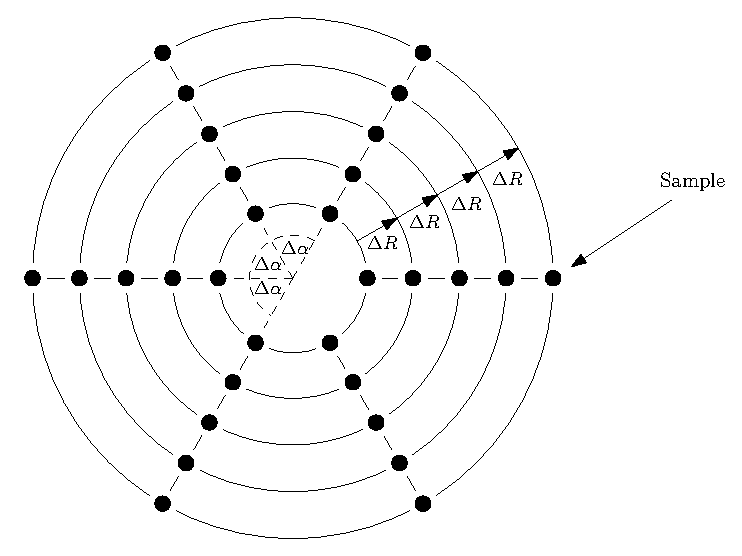
\includegraphics[scale=.8]{images/calibrationPatternTop.eps}
	\caption{Kalibrierungsmuster von oben mit $n = 5, m = 6$}
	\label{fig:calibrationPatternTop}
\end{figure}


\begin{figure}[!htb]
	\centering
	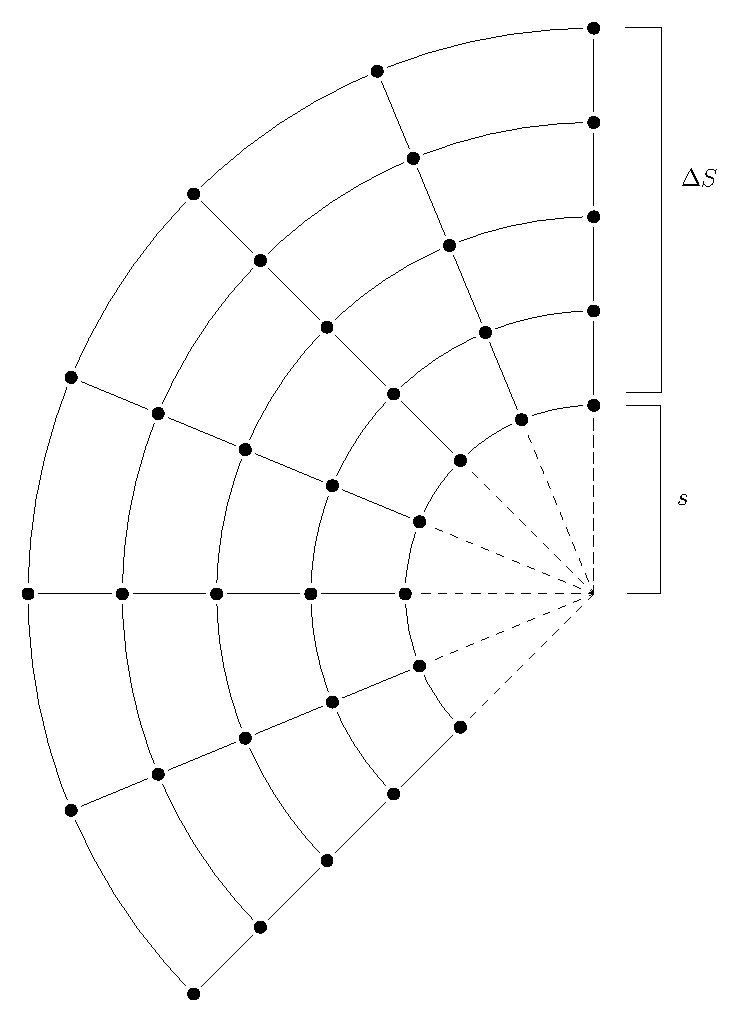
\includegraphics[scale=.7]{images/calibrationPattern2.eps}
	\caption{Kalibrierungsmuster entfaltet mit $n = 5, m = 6$}
	\label{fig:calibrationPattern}
\end{figure}

Zur Konstruktion des Musters benötigt man $\Delta S$ und $s$, die man aus der Geometrie des Kegels errechnen kann und außerdem den Öffnungswinkel, der gegeben ist als $\alpha = 2\pi\frac{R}{S}$ (siehe \ref{eq:paramLateral} in Kapitel \ref{s:cone}).

\subsection{Anzahl der Samples}
Die Anzahl der Samples sollte groß genug sein, um möglichst viel geometrische Informationen des Kegels zu erhalten, aber klein genug, dass eine Detektion der Samples problemlos möglich ist. Insbesondere auf dem innersten Kreis, macht sich eine zu hohe Sampleanzahl negativ bemerkbar, da der Abstand zueinander sehr klein wird, was eine Detektion erschwert. Des Weiteren sollte noch ein möglichst großer Teil der Kreislinien zu sehen bleiben, da diese für die Ellipsendetektion benötigt werden. 


\section{Intrinsische Kamerakalibrierung}
\label{s:intrinsic}
Bedingt durch die Wahl einer Weitwinkelkamera, enthält die Linse der Kamera eine starke tonnenförmige (nach außen gewölbte) Verzerrung (siehe Abbildung \ref{fig:calib}). Diese muss herausgerechnet werden, da sonst Abstände im Bild nicht mehr der Realität entsprechen und dadurch die Präzision der Entfaltung stark abnimmt (siehe Kapitel \ref{ch:analysis}). Es wird also zunächst eine Kamerakalibrierung durchgeführt, wobei wir nur an den intrinsischen Parametern, inklusive Verzerrungskoeffzienten, interessiert sind, um das Bild anschließend entzerren zu können. 


\begin{figure}[!htb]
	\centering
\begin{subfigure}{.5\textwidth}
	\centering
	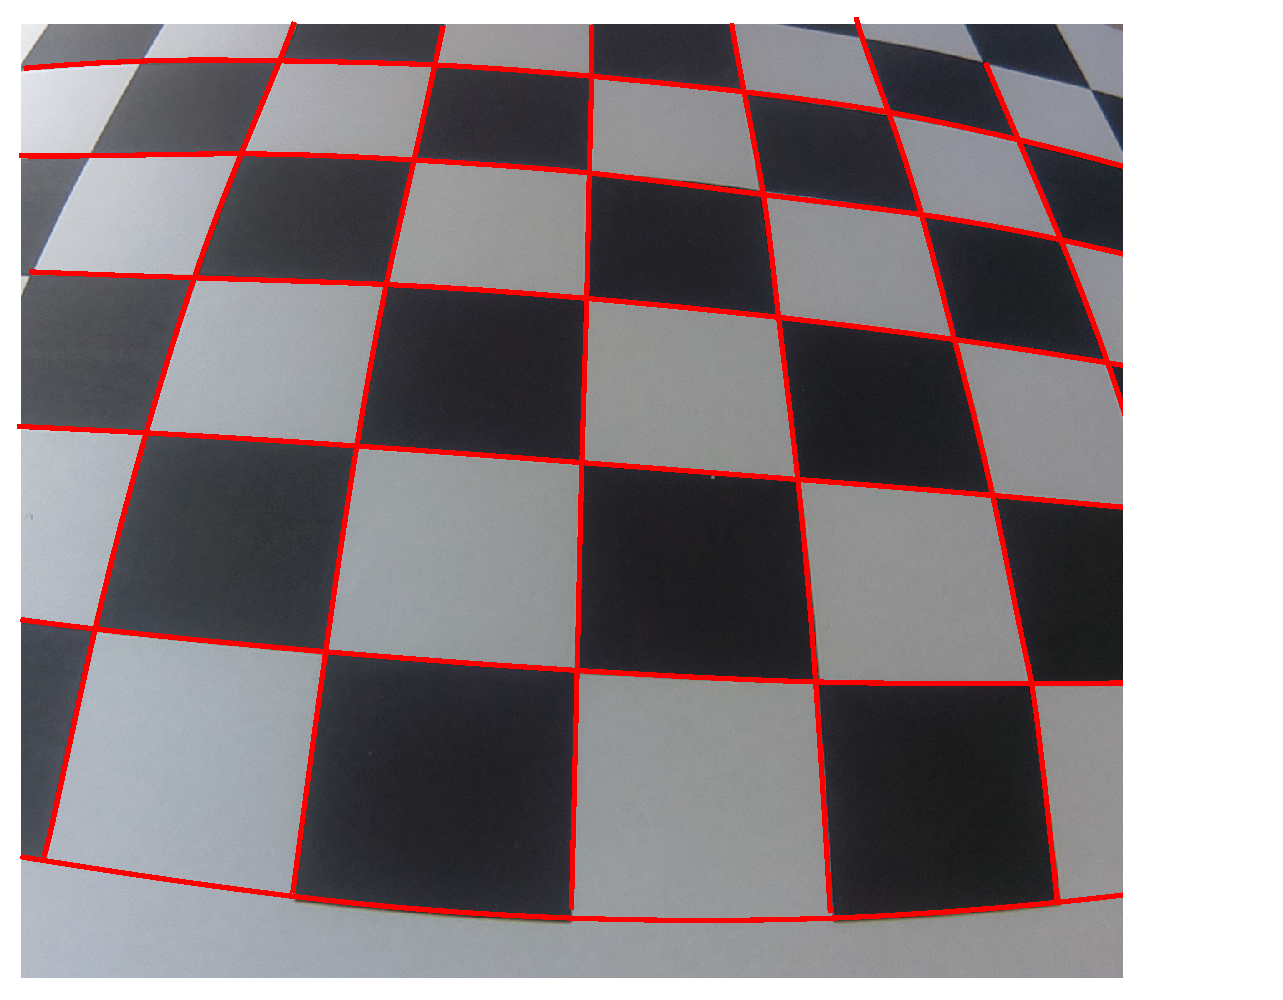
\includegraphics[scale=.35]{images/calibrationRaspi.eps}
	\caption{vor Kalibrierung}
	\label{fig:calibDist}
\end{subfigure}%
\begin{subfigure}{.5\textwidth}
	\centering
	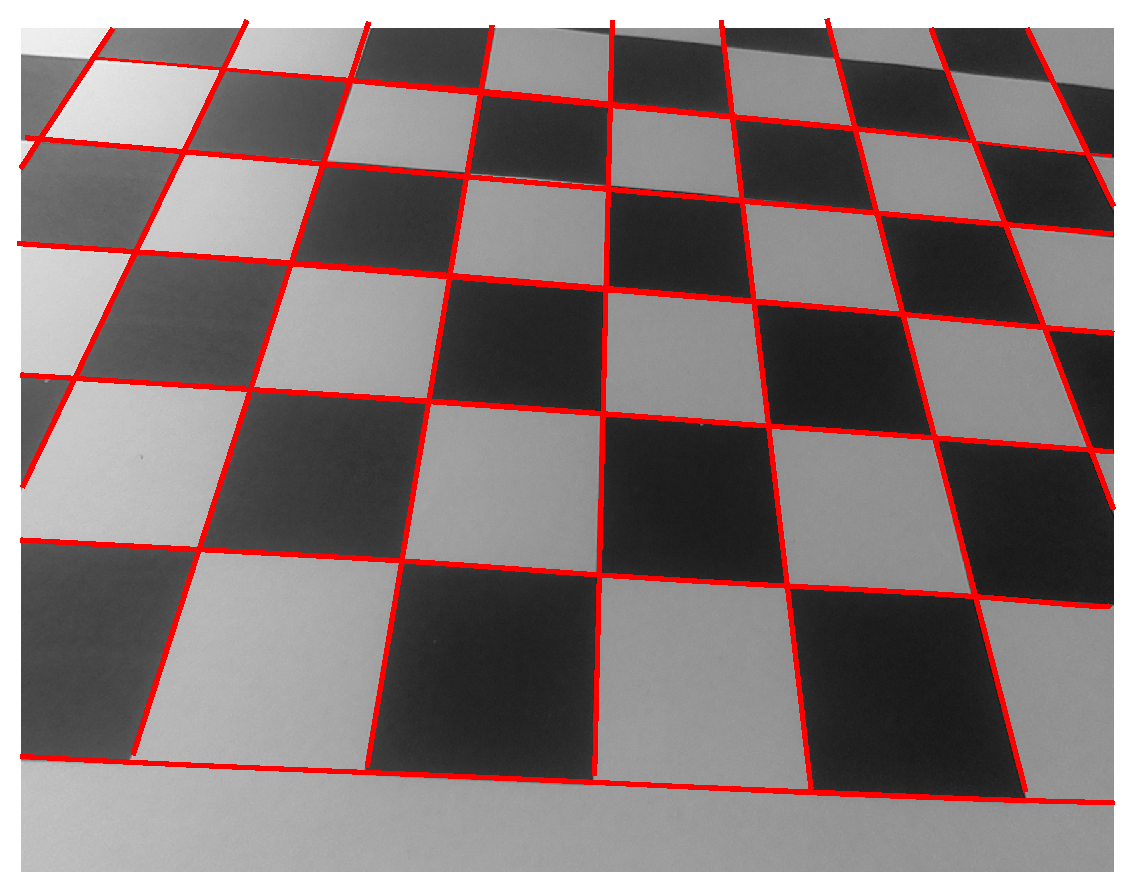
\includegraphics[scale=.4]{images/calibrationRaspi2.eps}
	\caption{nach Kalibrierung und Entzerrung}
	\label{fig:calibUndist}
\end{subfigure}
\caption{Kamerakalibrierung}
\label{fig:calib}
\end{figure}


\section{Detektion der charakteristischen Punkte}

Nach der Kamerakalibrierung und entsprechender Entzerrung werden die Bildkoordinaten der Samples bestimmt. Dazu wird ein Blob-Detektor (siehe Kapitel \ref{s:blob}) benutzt. 
Um ein Sample korrekt detektieren zu können, muss sich der Punkt farblich stark von seiner Umgebung abheben (siehe Definition: Blob \ref{def:blob}). Insbesondere dürfen die Kreislinien und Liniensegmente des Kalibrierungsmusters also nicht durchgezogen sein. Nach der Detektion werden die Blobs nach folgenden Kriterien gefiltert:

\begin{itemize}
	\item \textbf{Fläche:} zu kleine Blobs werden verworfen
	\item \textbf{Rundheit:} zu unrude Blobs werden verworfen. Rundheit ist hier definiert als $circ = \frac{4\pi\cdot \textrm{Fläche}}{\left(\textrm{Umfang}\right)^2}\in[0,1]$, wobei also ein Kreis mit $circ = 1$ maximal rund ist. 
	\item  \textbf{Konvexität:} zu unkonvexe Blobs werden verworfen. Konvextität ist hier definiert als $conv = \frac{\textrm{Fläche Blob}}{\textrm{Fläche konvexe Hülle}}$
\end{itemize}

In Abbildung \ref{fig:blobDetect} ist beispielhaft links ein Grauwertbild und rechts die detektierten Blobs (grün) auf dem gleichen Bild nach der Kameraentzerrung zu sehen.


\begin{figure}[!htb]
	\centering
	\begin{subfigure}{.5\textwidth}
		\centering
		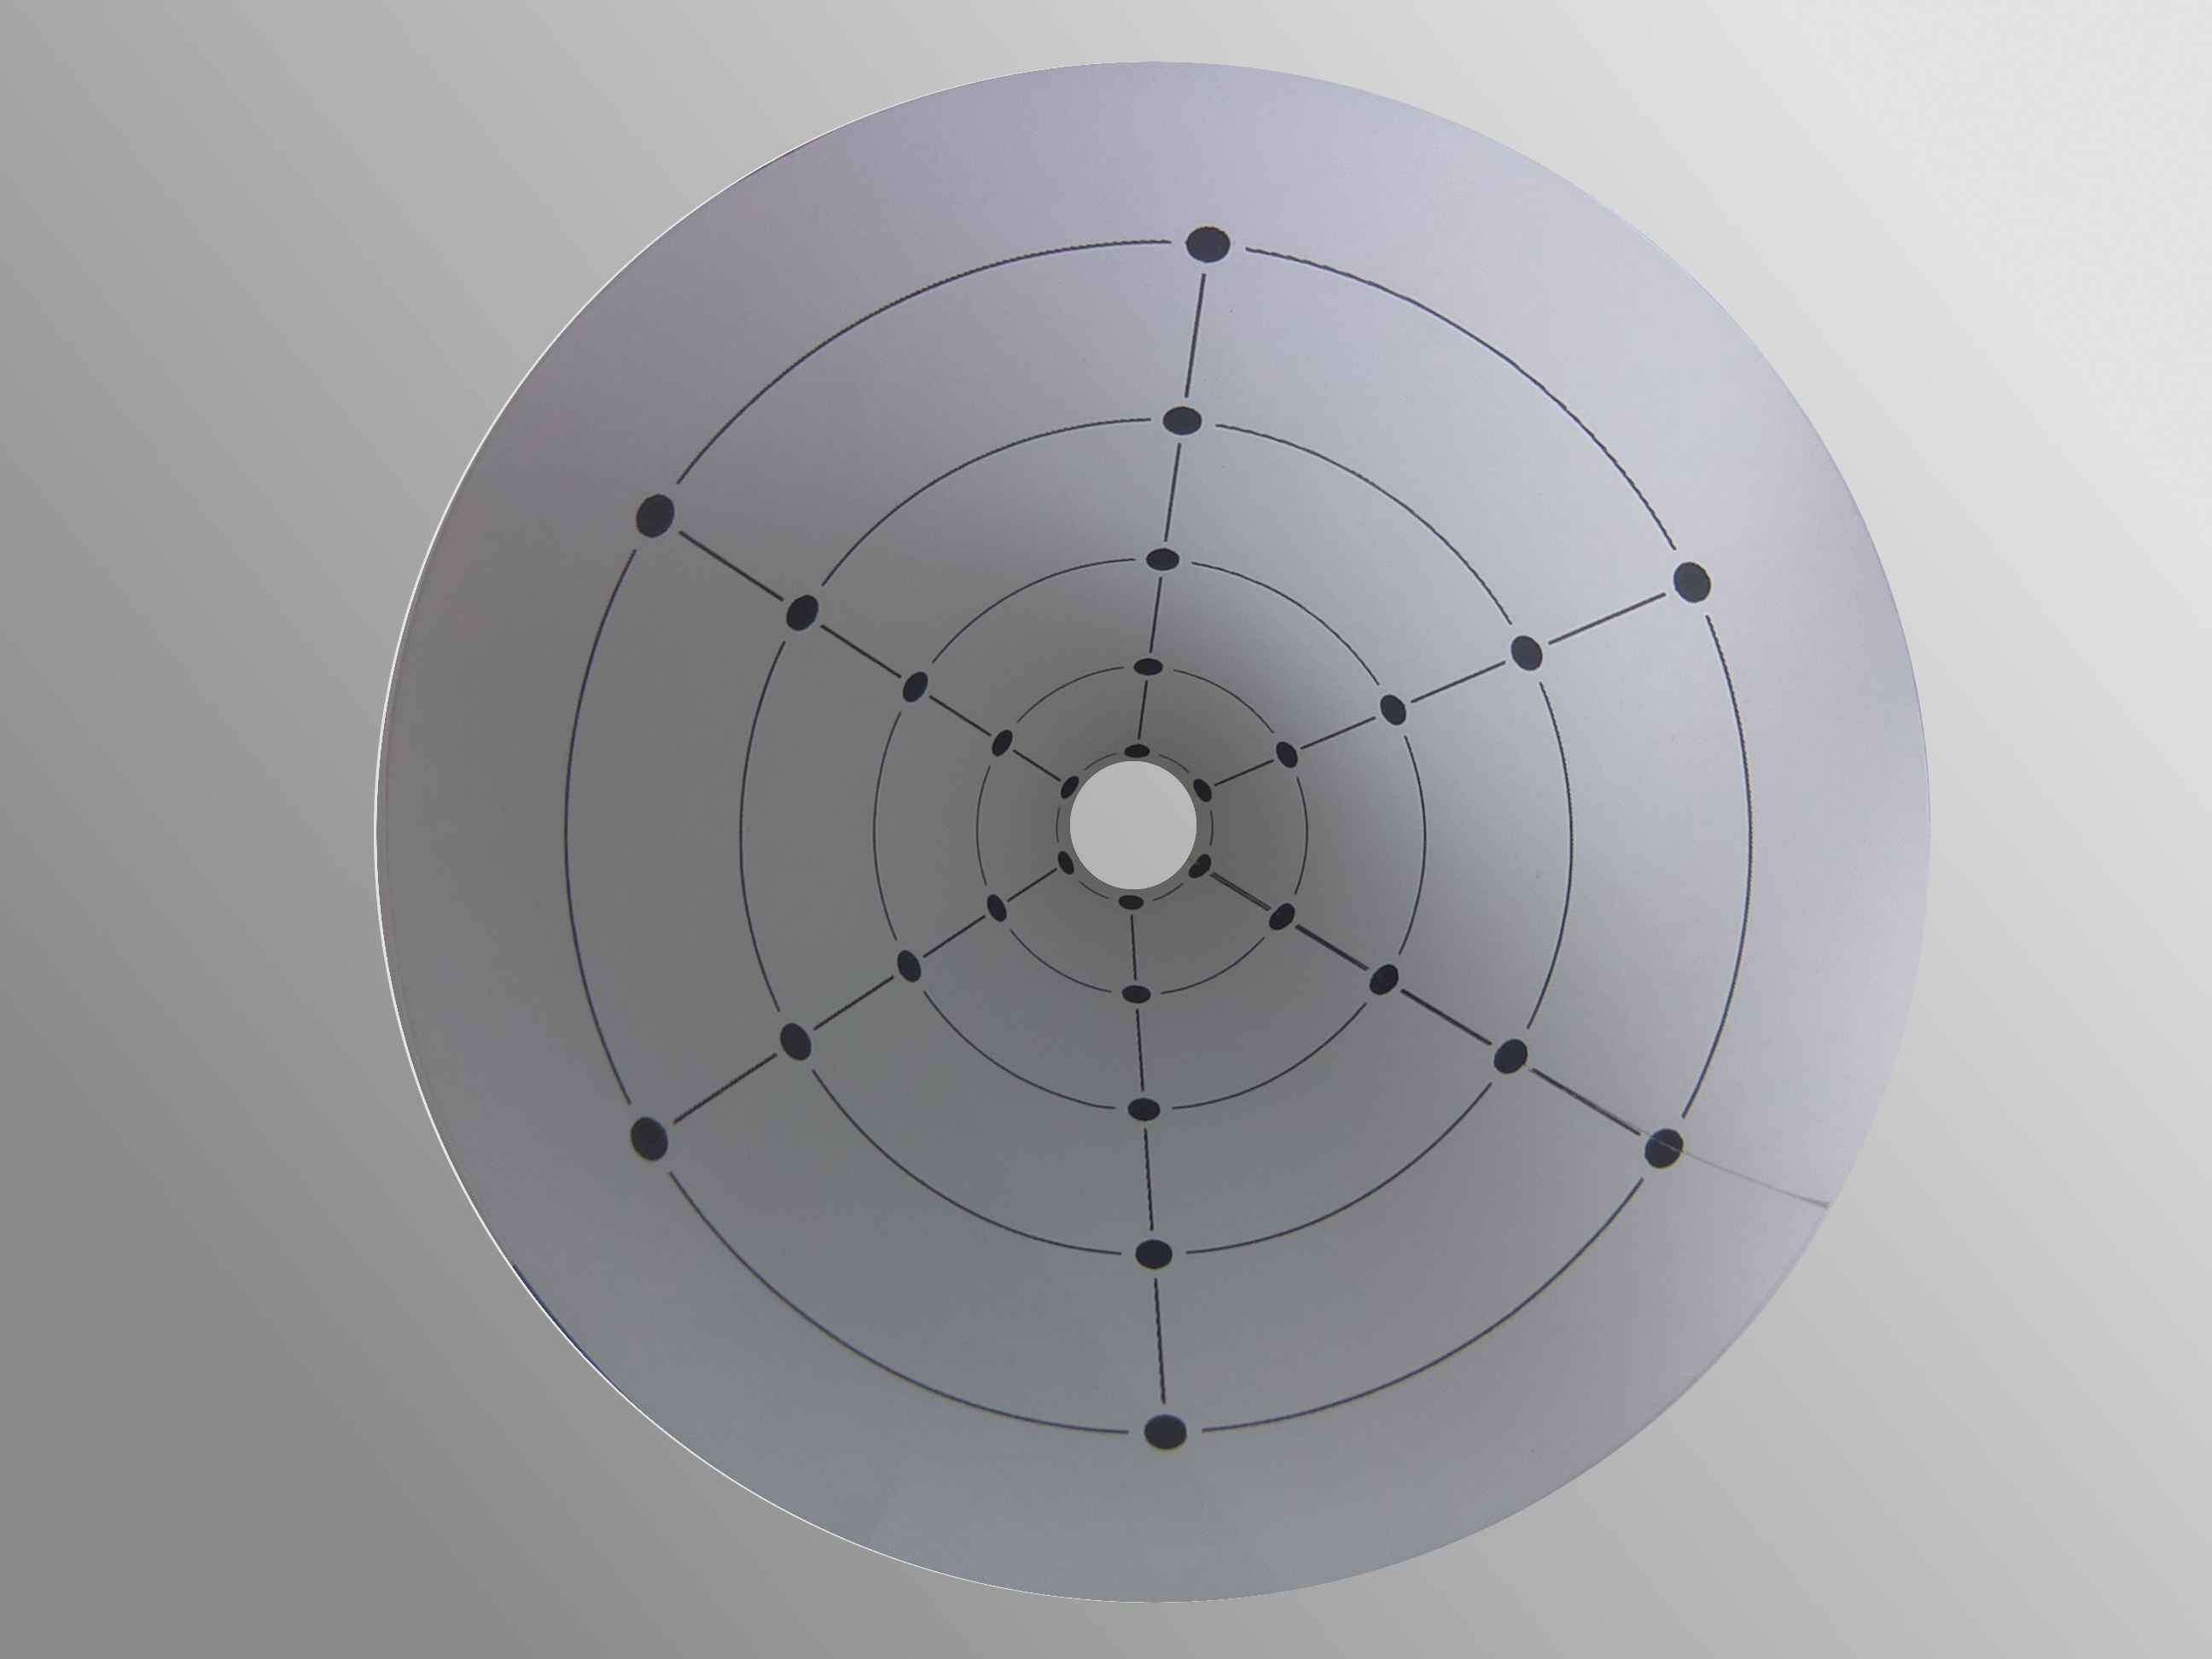
\includegraphics[width=.9\textwidth]{images/coneRasp.jpg}
		\caption{Grauwertbild}
	\end{subfigure}%
	\begin{subfigure}{.5\textwidth}
		\centering
		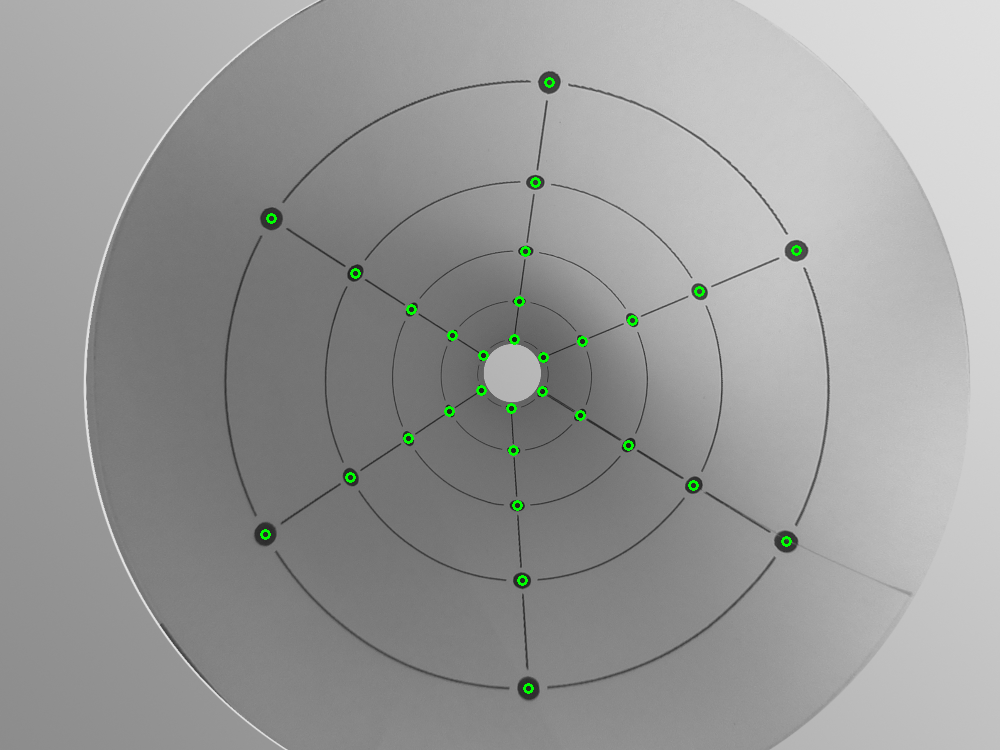
\includegraphics[width=.9\textwidth]{images/coneRaspDetectedDots.png}
		\caption{detektierte Blobs in grün}
	\end{subfigure}
	\caption{Detektion der Samples}
	\label{fig:blobDetect}
\end{figure}


\section{Ellipsen-Detektion}
\label{s:ellipseDetection}

\subsection{RANSAC}
Nachdem die Sample-Positionen bestimmt wurden, muss für jeden Sample entschieden werden, auf welcher der Kreislinien er liegt. Da die Kreise, bedingt durch perspektivische Verzerrung, zu  Ellipsen werden, wird eine Verfahren 
benötigt, dass Ellipsen erkennt. 

Zunächst werden die Kanten mit Hilfe von Canny (siehe Kapitel \ref{s:canny}) detektiert (siehe Abbildung \ref{fig:canny}). 

\begin{figure}[!htb]
	\centering
	\begin{subfigure}{.5\textwidth}
		\centering
		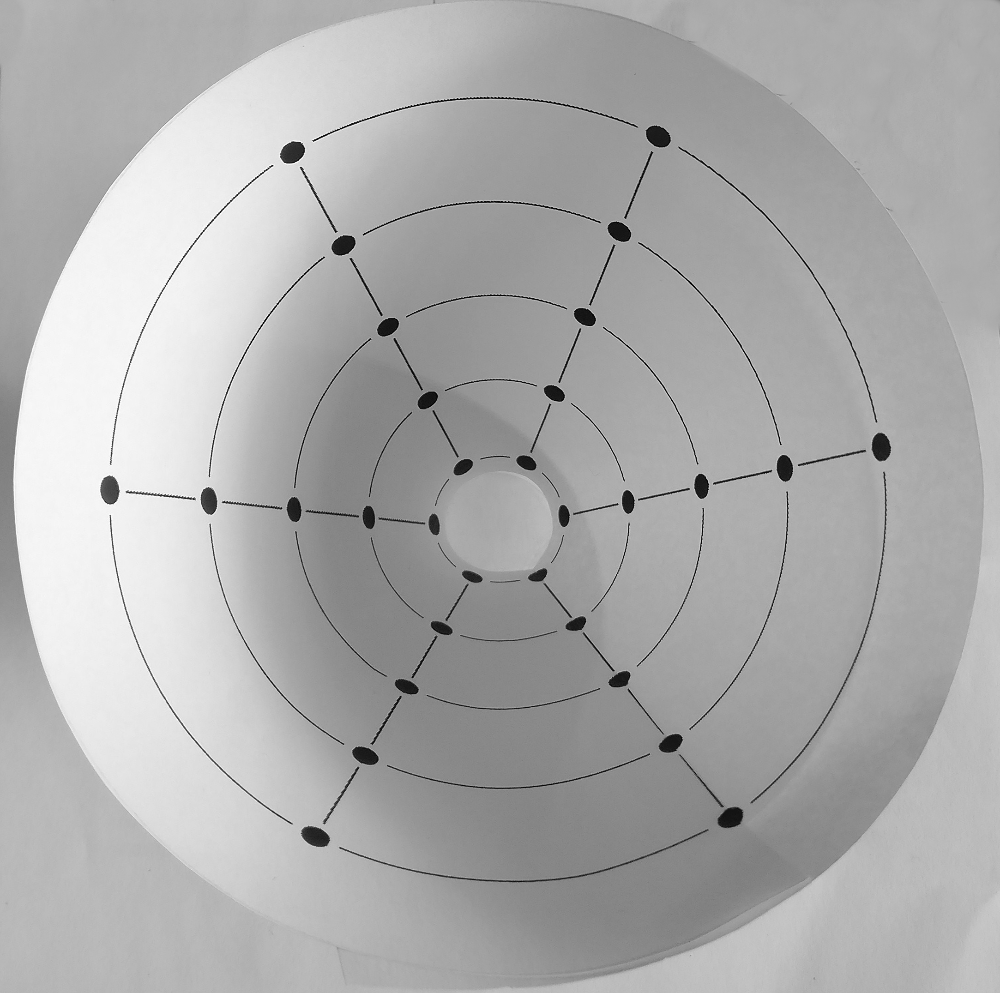
\includegraphics[width=.9\textwidth]{images/grey.png}
		\caption{Grauwertbild}
		\label{fig:beforeCanny}
	\end{subfigure}%
	\begin{subfigure}{.5\textwidth}
		\centering
		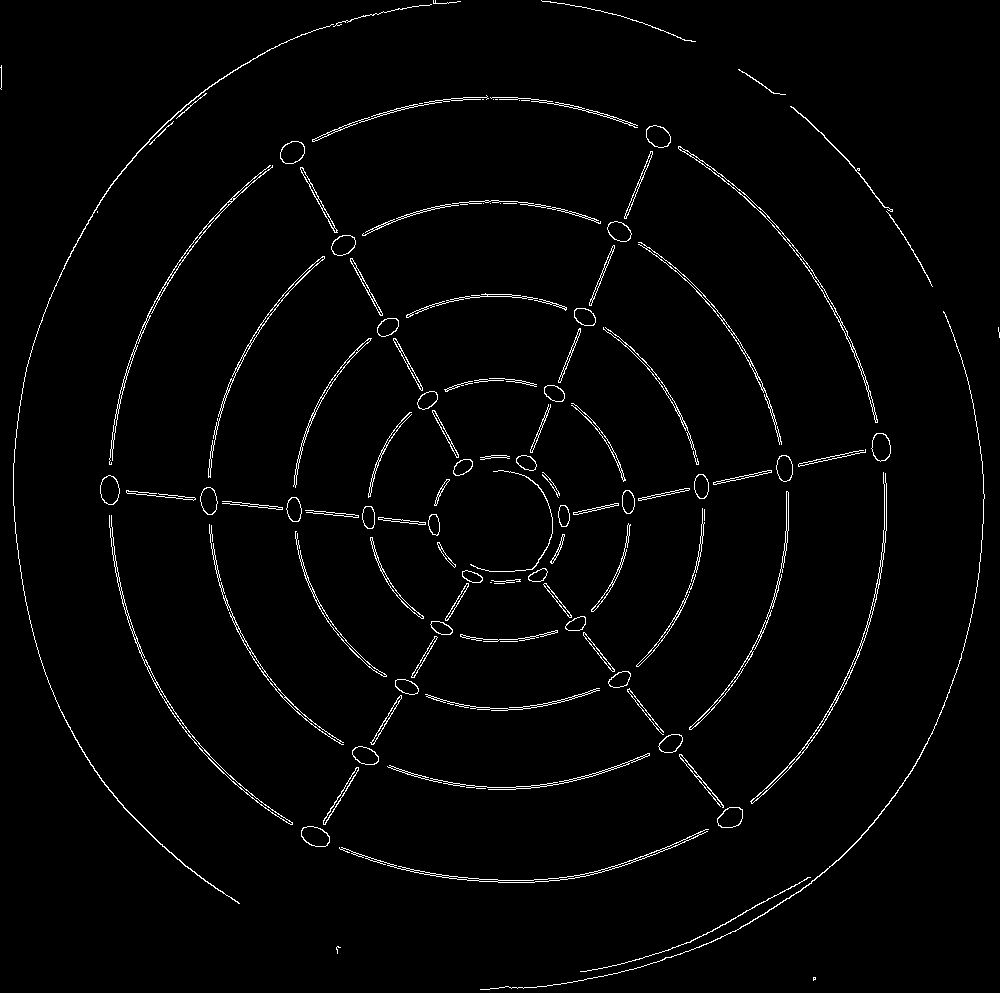
\includegraphics[width=.9\textwidth]{images/canny.png}
		\caption{Canny-Kanten}
		\label{fig:afterCanny}
	\end{subfigure}
	\caption{Canny-Kantendetektion auf Grauwertbild}
	\label{fig:canny}
\end{figure}

Anschließend versuchen wir möglichst genau das Zentrum der innersten Ellipsen zu schätzen.
Wir benutzen dafür Hough-Transformationen (siehe Kapitel \ref{s:hough}), um Linien im Kantenbild zu detektieren.
Es werden anschließend die Schnittpunkte aller Liniensegmente bestimmt. Bedingt durch Ungenauigkeiten beim Ausschneiden und Zusammenlegen im Kegel und perspektivischer Verzerrung, schneiden sich nicht alle Liniensegmente in einem Punkt.
Darüber hinaus werden, auf Grund der Liniendicke auf dem Kalibrierungsmuster, durch Canny viele Linien als doppelt Linien gekennzeichnet\footnote{Dies ist kein Widerspruch zur Eindeutigkeit von Canny-Kanten (siehe \ref{s:canny}). Stellt man sich ein relativ breites Liniensegment vor, so gibt es einmal den Übergang vom Hintergrund auf die Linie, sowie den Übergang von der Linie wieder auf den Hintergrund}. Auch ein inhomogener Hintergrund, erschwert die Schnittpunktsbestimmung. Um also möglichst robust einen Kandidaten auszuwählen, wird zuerst der Median der $x$-Koordinaten der Schnittpunkte und dann der Median der $y$-Koordinaten bestimmt. Die erhaltenen Koordinaten bilden den Schnittpunkt (siehe Abbildung \ref{fig:houghLines}).

\begin{figure}[!htb]
	\centering
	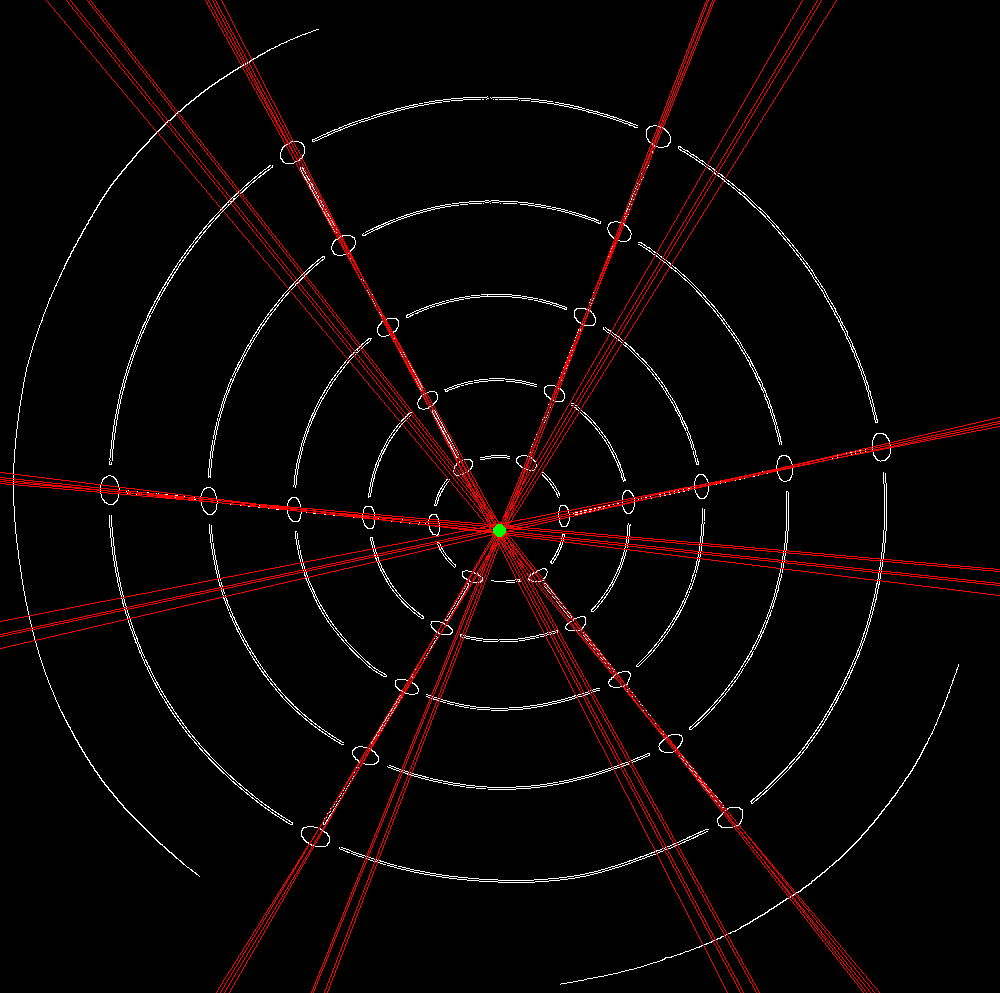
\includegraphics[scale=.25]{images/houghLines.png}
	\caption{Hough-Transformation zur Linien-Detektion (in rot gekennzeichnet) und bestimmter Schnittpunkt (in grün) }
	\label{fig:houghLines}
\end{figure}

Von diesem Schnittpunkt aus werden, in einer vorher definierte Anzahl, gleichmäßig, in alle Richtungen Strahlen ausgesendet.
Trifft ein Strahl ein weißes Pixel, wird dessen Position gekennzeichnet, trifft er den Rand des Bildes, wird er ignoriert. In Abbildung \ref{fig:rayCastWOE} sind die getroffenen weißen Pixel und der zugehörige Aussendepunkt eingezeichnet. 

\begin{figure}[!htb]
	\centering
	\begin{subfigure}{.5\textwidth}
		\centering
		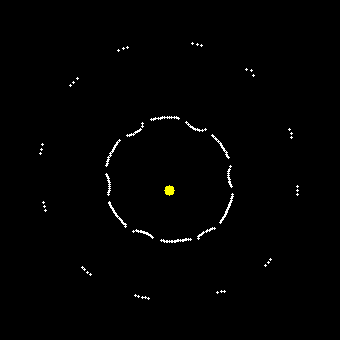
\includegraphics[width=.9\textwidth]{images/rayCast0.png}
		\caption{bestimme Pixel-Positionen}
		\label{fig:rayCastWOE}
	\end{subfigure}%
	\begin{subfigure}{.5\textwidth}
		\centering
		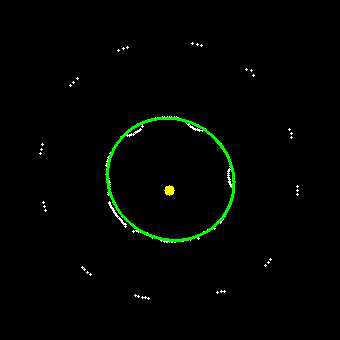
\includegraphics[width=.9\textwidth]{images/rayCast0Ellipse.png}
		\caption{bestimme Ellipse (grün)}
		\label{fig:rayCastWE}
	\end{subfigure}
	\caption{Ellipsendetektion: bestimme Pixel-Positionen (weiß), Aussendepunkt (gelb)}
	\label{fig:rayCast}
\end{figure}

Mit Hilfe der Postionen der weißen Pixel, wird anschließend durch RANSAC (siehe Kapitel \ref{s:ransac}) eine Ellipse geschätzt. 

Es wird konkret für sechs zufällig ausgewählte Punkte das lineare Gleichungssystem
\[
\begin{pmatrix}
x_1^2 & y_1^2 & x_1y_1 & x_1 & y_1 & 1\\
\vdots &\vdots & \vdots & \vdots &\vdots & \vdots\\
\vdots &\vdots & \vdots & \vdots &\vdots & \vdots\\
x_6^2 & y_6^2 & x_6y_6 & x_6 & y_6 & 1
\end{pmatrix} \begin{pmatrix}
a \\ b \\ c \\ d \\ e \\ f
\end{pmatrix} = \begin{pmatrix}
0 \\ 0 \\ 0 \\ 0 \\ 0 \\ 0
\end{pmatrix}
\]

gelöst, was auf der Gleichung \ref{eq:ellipseQuadratic} aus Kapitel \ref{s:ellipse} basiert. Nach dem Lösen wird geprüft, ob es sich tatsächlich um eine Ellipse handelt und mittels Hauptachsentransformation (siehe Kapitel \ref{s:ellipse}) in die Ellipsenform $(x_0,y_0,a,b,\phi)$ umgewandelt. Wir verwerfen anschließend Ellipsen mit, dessen Hauptachse wesentlich größer ist, als ihre Nebenachse, da wir eher wenig gestauchte Ellipsen erwarten. 


Um die, für RANSAC benötigte, Distanz zu berechnen, wird das Verfahren aus Kapitel \ref{sc:distPointEllipse} genutzt, was die exakte euklidische Distanz eines Punktes zu einer Ellipse approxmiert. 
Ein Verfahren wie das Verfahren der kleinsten Quadraten anstelle von RANSAC funktioniert hier nicht, da die weißen Pixel bezüglich einer zu bestimmenden Ellipse, ausreißerbehaftet sind. Wird zum Beispiel auf Grund schlechter Lichtverhältnisse eine Kreislinie nicht deutlich aufgenommen, kann es in dem Kantenbild (Abbildung \ref{fig:canny}) zu "`Löchern"' in den Kreislinien kommen und folglich treffen die ausgesendeten Strahlen die nächst äußere Kreislinie (siehe Abbildung \ref{fig:rayCastR}). 

Da die Laufzeit nicht im Vordergrund steht, kann eine großzügige Schätzung des Fehleranteils von $\epsilon = 0.4$ mit einer gewünschten Wahrscheinlichkeit $p = 0.9999$ gewählt werden, was zu einer Mindestanzahl an Iterationen von circa $200$ führt (siehe Kapitel \ref{s:ransac}). Die letztendlich bestimmten Ellipsen sind beispielhaft in Abbildung \ref{fig:detectedEllipses} zu sehen.  


\begin{figure}[!htb]
	\centering
	\begin{subfigure}{.5\textwidth}
		\centering
		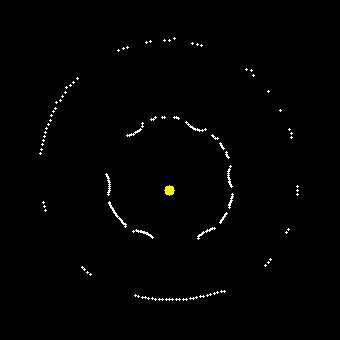
\includegraphics[scale=.6]{images/rayCastRobust.png}
		\caption{bestimme Pixel-Positionen}
		\label{fig:rayCastRWOE}
	\end{subfigure}%
	\begin{subfigure}{.5\textwidth}
		\centering
		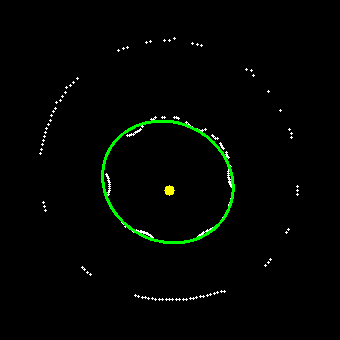
\includegraphics[scale=.6]{images/rayCastRobustEllipse.png}
		\caption{bestimme Ellipse (grün)}
		\label{fig:rayCastRWE}
	\end{subfigure}
	\caption{Ellipsendetektion bei Ausreißern}
	\label{fig:rayCastR}
\end{figure}


\begin{figure}[!htb]
	\centering
	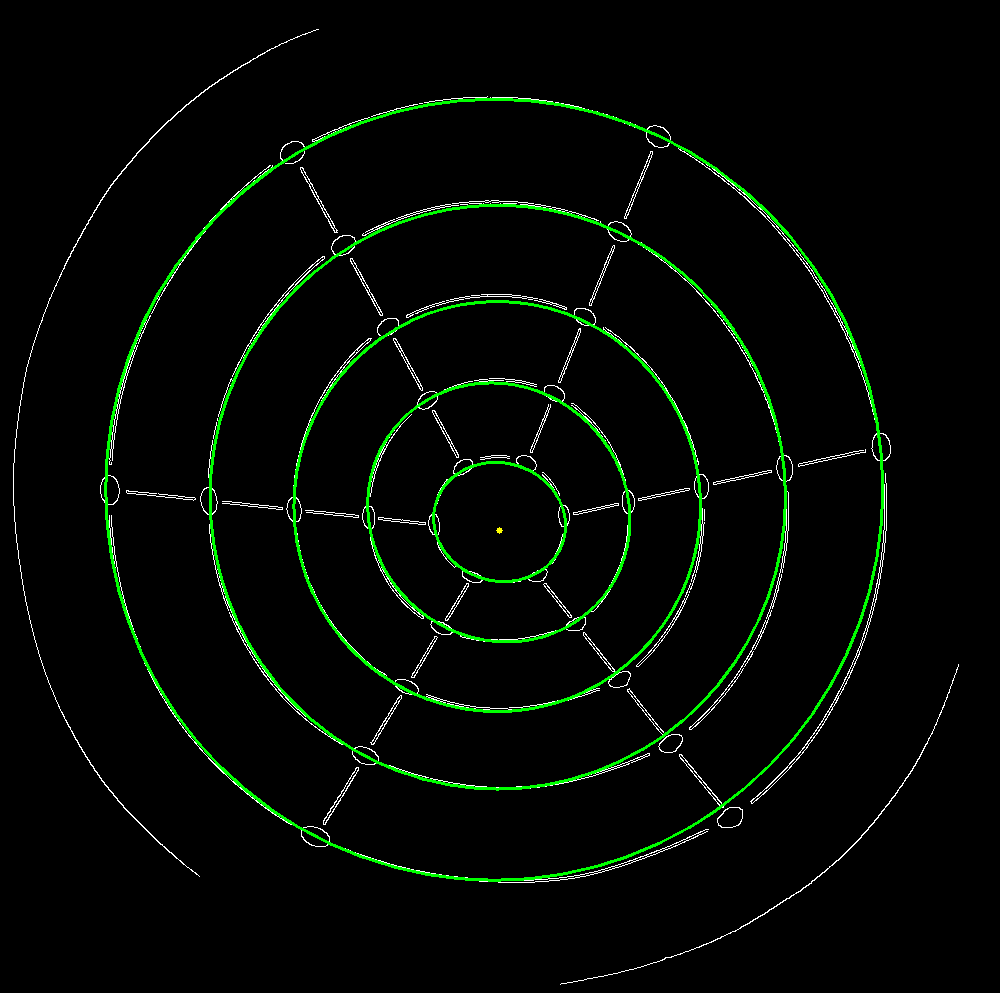
\includegraphics[scale=.25]{images/detectedEllipses.png}
	\caption{detektierte Ellipsen}
	\label{fig:detectedEllipses}
\end{figure}


\subsection{Analytical Deformable Templates}

Als Alternative zu RANSAC kann man die Ellipsen auch mittel \textit{Analytical Deformable Templates} (siehe Kapitel \ref{s:anaDef}) detektieren. Wir betrachten dazu folgende Funktion, deren Nullstellen wie in Kapitel \ref{s:ellipse}, eine um $\theta$ gedrehte Ellipse, mit Zentrum $(x_0,y_0)$ und Haupt- und Nebenachse $a$ und $b$ beschreiben. 
\begin{equation*}
	G(x,y) = \frac{((x - x_0)\cos\theta + (y - y_0)\sin\theta)^2}{a^2} + \frac{((x - x_0)\sin\theta - (y - y_0)\cos\theta)^2}{b^2} - 1
\end{equation*}

Wir konstruieren eine Energiefunktion:
\begin{equation*}
	E = E_M + E_A + E_S,
\end{equation*}
die sich zusammensetzt aus einem Term $E_M$, der die Kantenstärke auf dem Ellipsenrand maximiert, sowie einem Term $E_A$ der die Winkelähnlichkeit zwischen Ellipsennormale und Gradientenrichtung maximiert. Darüber hinaus fügen wir einen Term $E_S$ hinzu, der die Ellipse schrumpfen lässt. 

Genauer sehen die Terme wie folgt aus
\begin{equation*}
	\begin{aligned}
		E_M &= -\alpha\frac{1}{n}\sum_{i=0}^{n-1}I_M(p_i) \\
		E_A &= \beta\frac{1}{n}\sum_{i=0}^{n-1}\left(I_O(pi) - \atant{\left(\frac{\partial G}{\partial y}(p_i), \frac{\partial G}{\partial x}(p_i)\right)}\right)^2 \\
		E_S &= \gamma\frac{1}{n}\sum_{i=0}^{n-2}\abs{p_i - p_{i+1}},
	\end{aligned}
\end{equation*}

wobei $n$ die Anzahl der Punkte auf dem Ellipsenrand sind. $p_i$ ist definiert als der $i$-te Punkt auf der Ellipse (siehe parametrische Darstellung einer Ellipse).
Man wählt dabei als Startwert eine Ellipse, deren Zentrum dem Bildzentrum entspricht und deren Hauptachse und Nebenachse möglichst größ sind und bestimmt dann numerisch, beispielsweise durch Gradient Descent, ein Minimum der Funktion. Der Term $E_M$ wird minimal, wenn entlang der Ellipse die Kantenstärke (\textit{\textbf{M}agnitude}) groß ist. Der Term $E_A$ wird minimal wenn die Winkel der Normalenvektoren ähnlich zu denen der Kanten sind (\textit{\textbf{A}ngle}) und $E_S$ wird minimal, wenn die Distanz aufeinanderfolgender Ellipsepunkte klein wird, also die Ellipse als ganzes klein wird (\textit{\textbf{S}ize}). Der Term lässt die Ellipse also schrumpfen. $\alpha, \beta$ und $\gamma$ steuern hierbei den Einluss der einzelnen Terme. Das Minimum der Funktion sollte die äußerste Ellipse im Kalibirierungsmuster sein. Anschließend wird diese Ellipse vom Bild entfernt und man sucht wiederholt Minima der Funktion bis alle Ellipse detektiert wurden. 




\section{Zuordnung der Punkte}
\label{s:pointMapping}
Nach der Bestimmung der Ellipsen muss jede Sample-Positionen der zugehörigen Kreislinie, sowie Liniensegment zugeordnet werden, um seine Position auf dem Kegel bestimmen zu können. 
Zunächst wird für jeden Punkt diejenige Kreislinie ausgewählt, dessen zugehörige Ellipse die kürzeste Distanz zu ihm hat (siehe Abbildung \ref{fig:ellipseMapping}).

Mit Hilfe dieser Zuordnung können die Ellipsen aus Kapitel \ref{s:ellipseDetection} erneut geschätzt werden. Diesmal wird das Verfahren der kleinsten Quadrate genutzt, da nur die ausreißerfreihen Samples als Messdaten dienen und wir eine optimale Lösung für alle Samples anstreben.  

Um nun die Samples auch ihren Liniensegmenten zuzuordnen, wird zunächst der Mittelpunkt der Samples auf der innersten Ellipse bestimmt. Anschließend werden die Samples auf der innersten Ellipsen nach dem Winkel der Verbindungslinien zwischen Sample und Mittelpunkt mit der $X$-Achse sortiert. 
Die restlichen Samples können nicht nach dem gleichen Schema sortiert werden, da der bestimme Mittelpunkt nicht der genaue Schnittpunkt aller Liniensegmente ist. Der Mittelpunkt liegt also nicht auf der Verlängerung eines Liniensegments. Die Winkel der Verbindungslinien der Samples (auf einem gemeinsamen Liniensegment) und dem Mittelpunkt mit der $X$-Achse sind nicht identisch (siehe Abbildung \ref{fig:sampleMappingProblem}).

\begin{figure}[!htb]
	\centering
	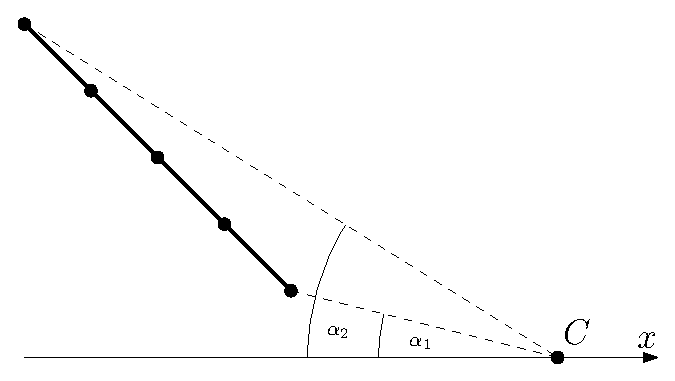
\includegraphics[scale=.9]{images/sampleMappingProblem.eps}
	\caption{Winkel zwischen Samples und Mittelpunkt $C$ sind nicht identisch}
	\label{fig:sampleMappingProblem}
\end{figure}

Stattdessen wird für jedes Sample auf den darauffolgenden Ellipsen das Sample auf der vorherigen Ellipse mit der kürzesten Distanz bestimmt. 
Die Samples können nun entsprechend sortiert werden. Die zugeordneten Liniensegmente sind exemplarisch in Abbildung \ref{fig:lineMapping} zu sehen. 


\begin{figure}[!htb]
	\centering
	\begin{subfigure}{.5\textwidth}
		\centering
		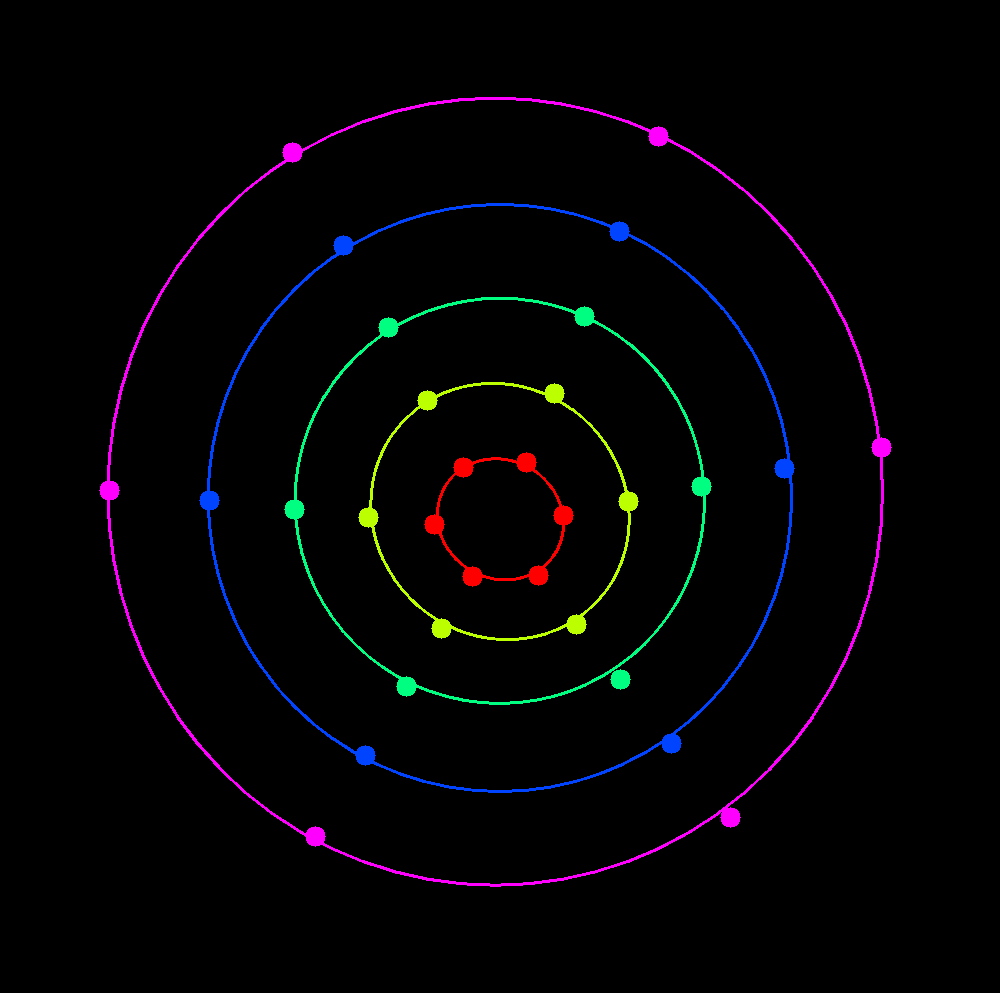
\includegraphics[width=.9\textwidth]{images/ellipseMapping.png}
		\caption{Zuordnung von Punkten zu Ellipsen}
		\label{fig:ellipseMapping}
	\end{subfigure}%
	\begin{subfigure}{.5\textwidth}
		\centering
		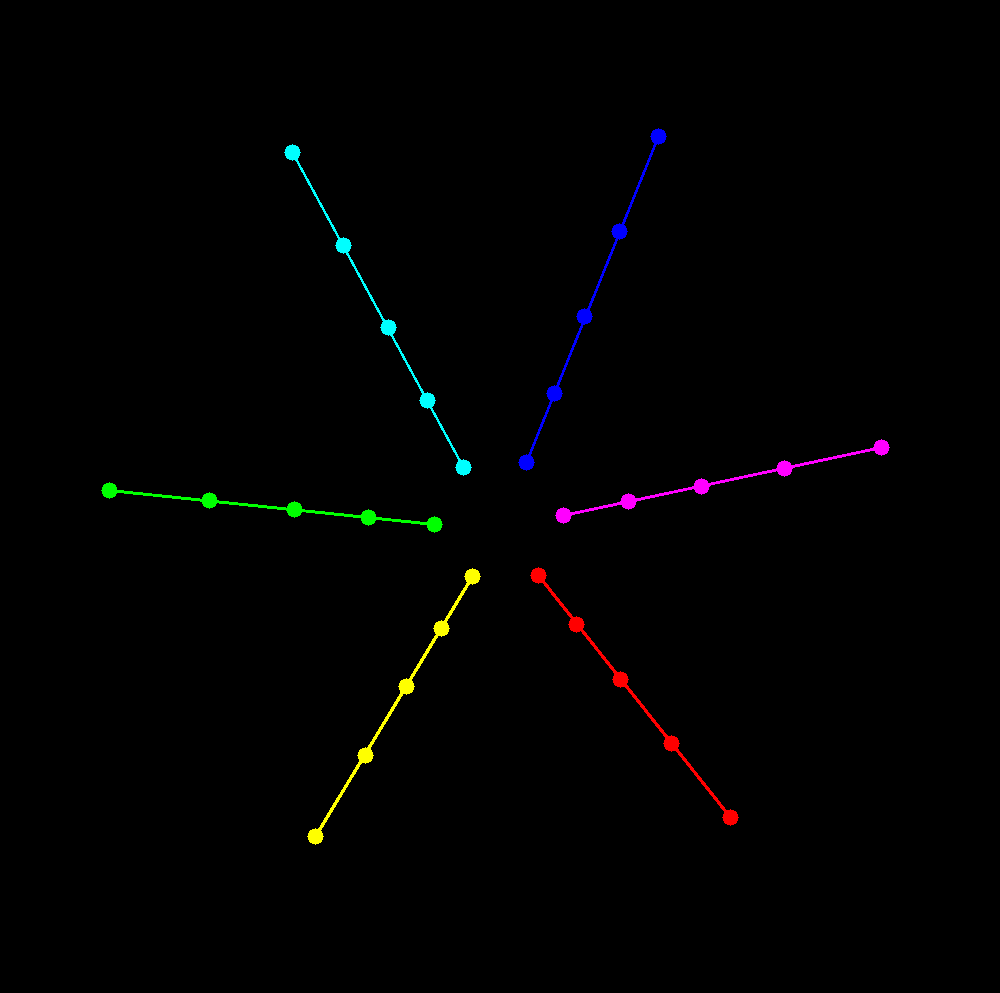
\includegraphics[width=.9\textwidth]{images/lineMapping.png}
		\caption{Zuordnung von Punkten zu Liniensegmenten}
		\label{fig:lineMapping}
	\end{subfigure}
	\caption{Zuordnung von Punkten zu Ellipsen (links) und Liniensegmenten (rechts)}
	\label{fig:mapping}
\end{figure}


\section{Weltkoordinaten bestimmen}

Mit Hilfe der Parametrisierung des Kegelstumpfs aus Kapitel \ref{s:canny} können wir die 3D-Koordinaten eines Samples folgendermaßen angeben:

Ohne Beschränkung der Allgemeinheit, seien die Ellipsen $i = 0,\dotsc,n - 1$ aufsteigend nach ihrer "`Größe"'\footnote{Etwas formaler, könnte man die Ellipsen hier nach ihrem Flächeninhalt sortieren. Für Ellipsen $E_0(x_0,y_0,a_0, b_0, \theta_0)$ und $E_1(x_1,y_1,a_1, b_1,\theta_1)$ gilt $E_0 \leq E_1$ g.d.w. $\pi\cdot a_0 \cdot b_0 \leq \pi \cdot a_1 \cdot b_1$} sortiert, so wie es das Verfahren in \ref{s:ellipseDetection} beschreibt.
Außerdem seien die Liniensegmente $j = 0,\dotsc,m - 1$ aufsteigend nach Winkel mit der $X$-Achse, wie in \ref{s:pointMapping} beschrieben, sortiert. 
Eine Sample kann also eindeutig durch ein Tupel $(i,j) \in [0,n-1]\times [0,m-1]$ identifiziert werden und $(x_{ij},y_{ij},z_{ij})$ bezeichne seine Koordinaten im Weltkoordinatensystem. 

Analog zur parametrischen Darstellung von Kegelstümpfen (Gleichung \ref{eq:paramFrustum}) in Kapitel \ref{s:cone} ergibt sich:

\begin{equation*}
\begin{aligned}
x_{ij} &= r_i~cos \theta_j \\
y_{ij} &= h_i\\
z_{ij} &= r_i~sin \theta_j
\end{aligned}
\end{equation*}
$\forall (i,j) \in [0,n-1]\times [0,m-1]$ mit 
\begin{equation*}
\begin{aligned}
r_i &= r + \frac{i}{n}\cdot(R - r) \quad&\forall i\in[0,n-1]\\
h_i &= \frac{i}{n}\cdot\Delta H &\forall i\in[0,n-1]\\
\theta_j &= \frac{j}{m-1} \cdot  2\pi  &\forall j\in[0,m-1]
\end{aligned}
\end{equation*}

\section{Entfaltung}
\label{s:unfolding}
Die eigentliche Entfaltung des Kegels kann mit zwei unterschiedlichen Ansätzen realisiert werden. 
Die erste Möglichkeit ist die \textit{Vorwärtsentfaltung}. Hierbei wird für jedes Pixel auf dem Kegelbild eine 3D-Koordinate durch geeignete Interpolation bestimmt und dann auf die Mantelfläche abgebildet. Beim zweiten Ansatz, der \textit{Rückwärtsentfaltung}, wird ein Punkt von der Mantelfläche zurück auf den Kegel abgebildet und von dort mit einer Projektionsmatrix auf die Bildebene projiziert und dann interpoliert. 

Im folgenden wird genauer auf beide Verfahren eingegangen, sowie deren Probleme erläutert.

\subsection{Vorwärtsentfaltung}
Bei der \textit{Vorwärtsentfaltung} muss wie oben erwähnt zu jedem Pixel die zugehörige 3D Koordinate im Weltkoordinatensystem berechnet werden. Da bisher jedoch nur die Positionen der Samples bekannt sind muss hier 

Zunächst betrachten wir diejenigen Pixel, die sich weder auf einer Kreislinie, noch auf einem Liniensegment befinden. Es gibt zu einem Pixel $P$ also immer vier Sample-Nachbarn $(bl, br, tr, tl)$. Diese Situation ist in Abbildung \ref{fig:radialInterpolation} illustriert. 

Nachdem die vier Nachbarn bestimmt wurden, können im ersten Schritt die Abstände $d_1$ und $d_2$ zu inneren Ellipse $E_b$, respektive äußeren Ellipse $E_t$ berechnet werden. Mithilfe dieser Abständen kann nun eine \textit{Interpolationsellipse}~$E_1$ definiert werden als
\begin{equation*}
	E_{int} = \left(\frac{d_1}{d_1 + d_2}\right) \cdot E_t + \left(\frac{d_2}{d_1 + d_2}\right) E_b,
\end{equation*}

wobei eine Multiplikation mit einem Skalar alle Charakteristika einer Ellipse skaliert. Der Drehwinkel $\theta$ wird hierbei bei $2\pi$ umgebrochen. Eine Addition geschieht elementweise. Im nächsten Schritt wird der Schnittpunkt $L$ mit dem Liniensegment $\overline{bltl}$, sowie der Schnittpunkt $R$ mit dem Liniensegment $\overline{brtr}$ bestimmt. 

Da sich $tl$, $L$ und $bl$ nun auf einem gemeinsamen Liniensegment befinden, kann bezüglich der Weltkoordinaten linear interpoliert werden. Analoges gilt für $tr$,$R$ und $br$. 

Die drei Punkte $(L, P, R)$ befinden sich auf der Interpolationsellipse und somit können die  Winkel $(\phi_L, \phi_P, \phi_R)$ bezüglich des gemeinsamen Ellipsenkoordinatensystems bestimmt werden. 

Analog zu oben werden die 3D-Koordinaten von $P$ als lineare Interpolation zwischen den gerade bestimmen 3D-Koordinaten von $L$ und $R$ bestimmt. Als Interpolationsfaktor benutzen wir
$\frac{\phi_L - \phi_P}{\phi_L - \phi_R}$


\begin{figure}[!htb]
	\centering
	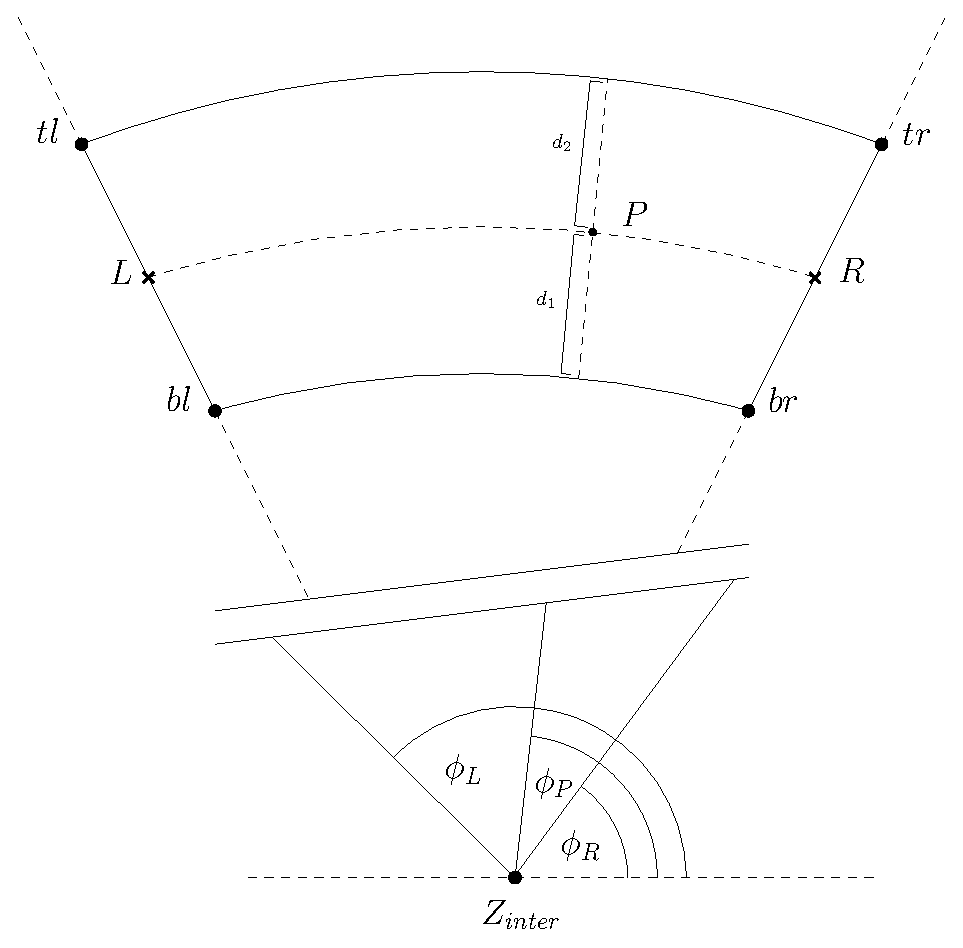
\includegraphics[scale=.6]{images/radialInterpolation.eps}
	\caption{Interpolation der 3D-Koordinaten}
	\label{fig:radialInterpolation}
\end{figure}


\begin{figure}[!htb]
	\centering
	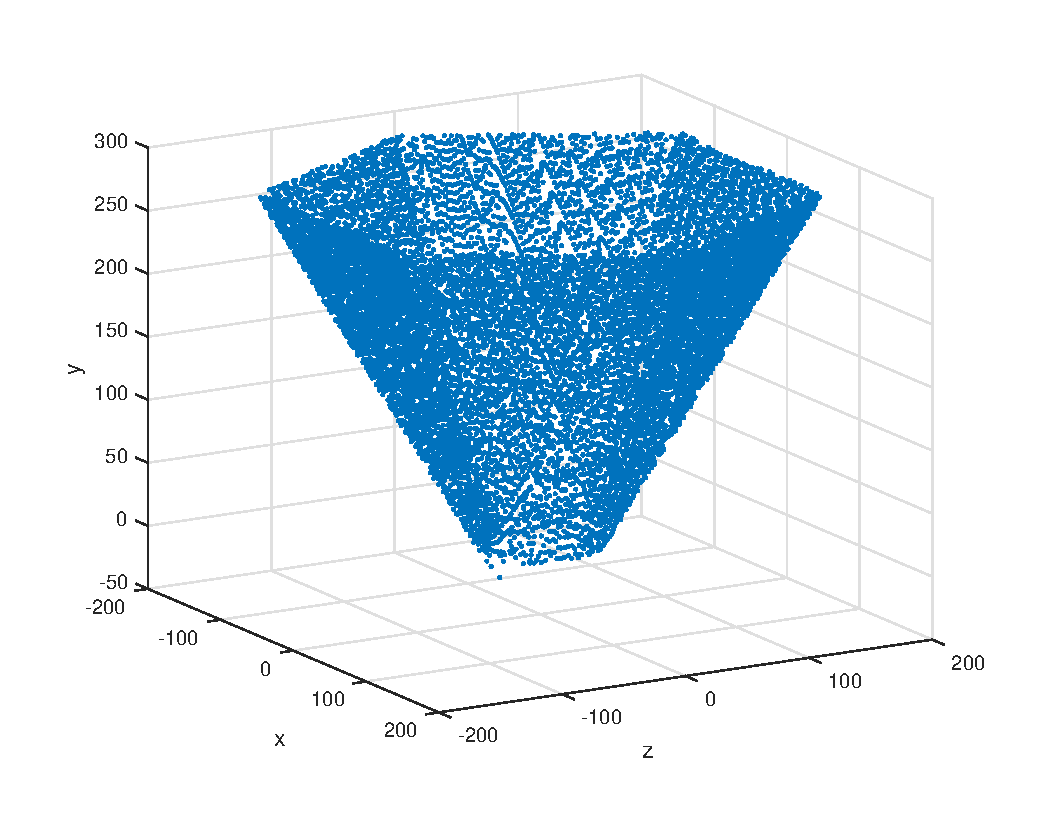
\includegraphics[scale=.7]{images/3d_interpol.eps}
	\caption{interpolierter Kegel}
	\label{fig:3DInterpol}
\end{figure}

Analog werden die auf Liniensegmenten befindlichen Punkte einfach linear interpoliert. Die Punkte, die sich auf Kreislinien befinden werden über Winkel interpoliert. 

Jedes Pixel hat nun 3D-Koordinaten im Kegel erhalten, die beispielhaft in Abbildung \ref{fig:3DInterpol} zu sehen sind.
Anhand der Abbildung lässt sich das erste Problem bei der Vorwärtsentfaltung feststellen. Zwischen den Samples auf einer Kreislinie sollten die interpolierte Positionen nach außen gewölbt sein, da ein Kegel rund ist. Da wir jedoch Interpolieren und nicht Extrapolieren, gehen die Werte nie über die zur Interpolation genutzten Werte hinaus. Konkreter kann eine interpolierte Position keine größeren oder kleineren $X$ und $Z$ Koordinaten erhalten, als die der genutzten Samples. Diese wäre jedoch notwendig, sodass die Rundung des Kegels erhalten bleibt. Die Oberfläche des Kegels scheint eckig. 

Neben der außerdem sehr hohen Laufzeit, bedingt durch die komplexe Interpolation, ergibt sich noch ein weiteres Problem, dass sich erst bei der Entfaltung ergibt. 

Die eigentliche Entfaltung geschieht über die Abbildung \ref{eq:coneToLateral}, die in Kapitel \ref{s:cone} konstruiert wurde. Die erhaltenen Werte müssen anschließend skaliert werden, da im entfalteten Bild sonst 1 mm einem Pixel entspreche. Es ergibt sich das entfaltete Bild, wie in Abbildung \ref{fig:forwardUnfold} dargestellt. Auch schon bei kleinen Skalierungen entstehen auffällige "`Löcher"' im entfalteten Bild. Grund dafür ist, dass jedes Pixel aus dem Ursprungsbild auf eine 2D-Koordinate der Mantelfläche abgebildet wird. Auch nach einer Skalierung handelt es sich bei diesen Werten im Allgemeinen nicht um ganzzahlige Werte. Es muss im entfalteten Bild gerundet werden. Auch wenn Rundungsfehler nicht entständen, fehlte es einfach an genügend Informationen, gerade in den inneren, kleineren Regionen des Ursprungsbild.

Da wir von dem Ursprungsbild aus auf das entfaltete Bild abbilden, ist außerdem eine Interpolation auf dem Ursprungsbild nicht möglich, da wir vorher nicht genau wissen, wo Löcher entstehen. Man müsste als entweder auf dem resultierendem Bild interpolieren (siehe Kapitel \ref{ch:summary}), oder zu gegebenen Löchern über die Umkehrabbildung auf dem Ursprungsbild interpolieren. 

\begin{figure}[!htb]
	\centering
	\begin{subfigure}{.5\textwidth}
		\centering
		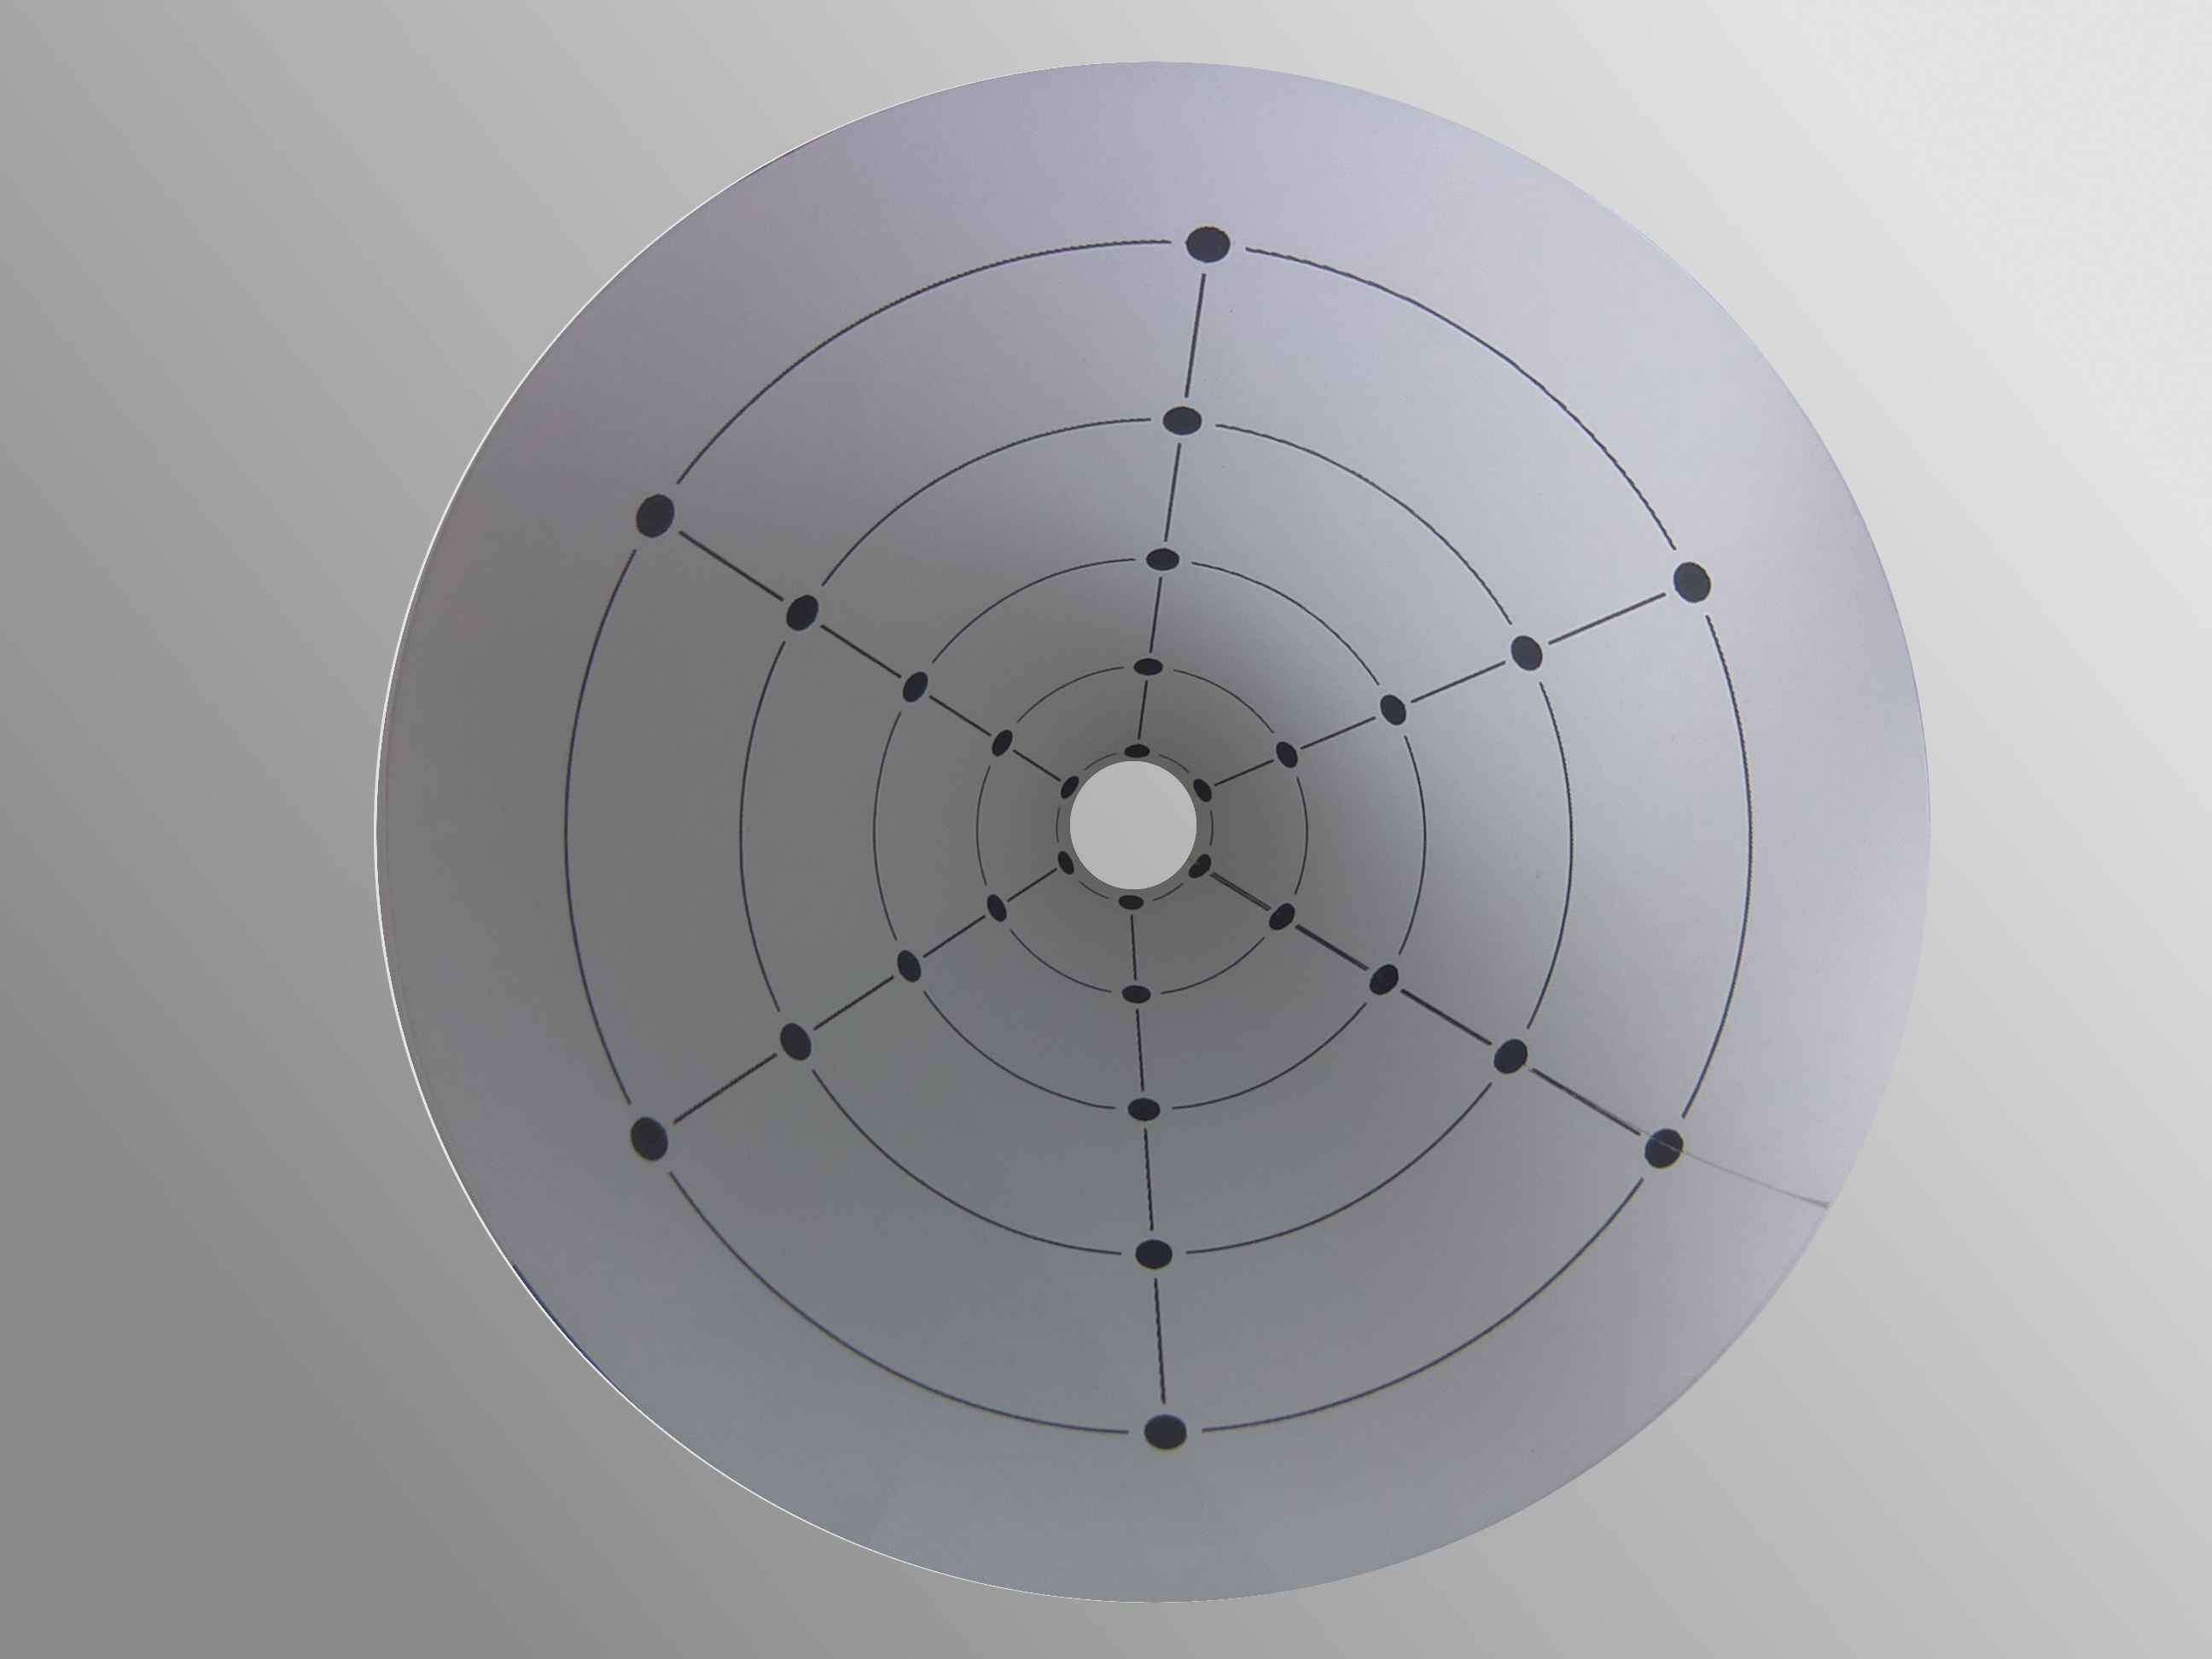
\includegraphics[width=.9\textwidth]{images/coneRasp.jpg}
		\caption{Ursprungsbild}
	\end{subfigure}%
	\begin{subfigure}{.5\textwidth}
		\centering
		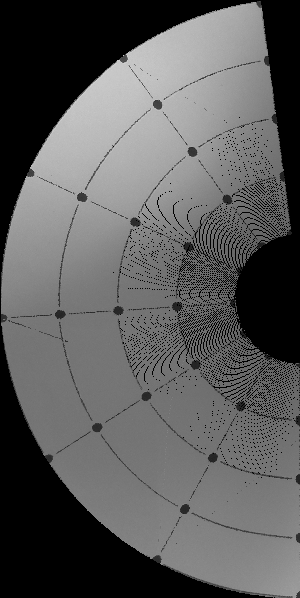
\includegraphics[angle=-90, width=.9\textwidth]{images/coneRaspUnWarpForward.png}
		\caption{entfaltetes Bild (um 90° im Uhrzeigersinn gedreht)}
	\end{subfigure}
	\caption{Vorwärtsentfaltung}
	\label{fig:forwardUnfold}
\end{figure}

Es bietet sich dann jedoch an, direkt die Umkehrabbildung zu nutzen, was die Motivation hinter der Rückwärtsentfaltung ist.

\subsection{Rückwärtsentfaltung}
Bei der Rückwärtsentfaltung gehen wir von dem entzerrten Bild aus, dessen geometrischen Eigenschaften aus der parametrischen Form der Mantelfläche des Kegels bekannt sind und versuchen rückwärts Pixelkandidaten im Ursprungsbild zu bestimmen. 

Zunächst bestimmen wir zu den gegebenen 3D-Korrespondenzen der Samples eine Projektionsmatrix wie in Kapitel \ref{s:calib} mittels \textit{Direct Linear Transformation}. Wir machen also eine Kamerakalibrierung, wobei die Kameraverzerrungen schon herausgerechnet wurden (siehe Kapitel \ref{s:intrinsic}). Wir erhalten somit eine Abbildung die aus den 3D-Koordinaten im Kegel auf Bildkoordinaten abbildet. 

Wir benutzen anschließend für jedes Pixel auf dem entzerrten Bild die Umkehrabbildung \ref{eq:LateralToCone} aus Kapitel \ref{s:cone}. Wir erhalten wieder 3D-Kegelkoordinaten. Die Projektionsmatrix kann nun einfach auf diese Punkte angewandt werden und wir erhalten Bildpunkte im Ursprungsbild. 

Die resultierenden Bildpunkte sind im Allgemeinen nicht ganzzahlig. Im Gegensatz zur Vorwärtsentfaltung kann hier jedoch einfach interpoliert werden. 


\begin{figure}[!htb]
	\centering
	\begin{subfigure}{.5\textwidth}
		\centering
		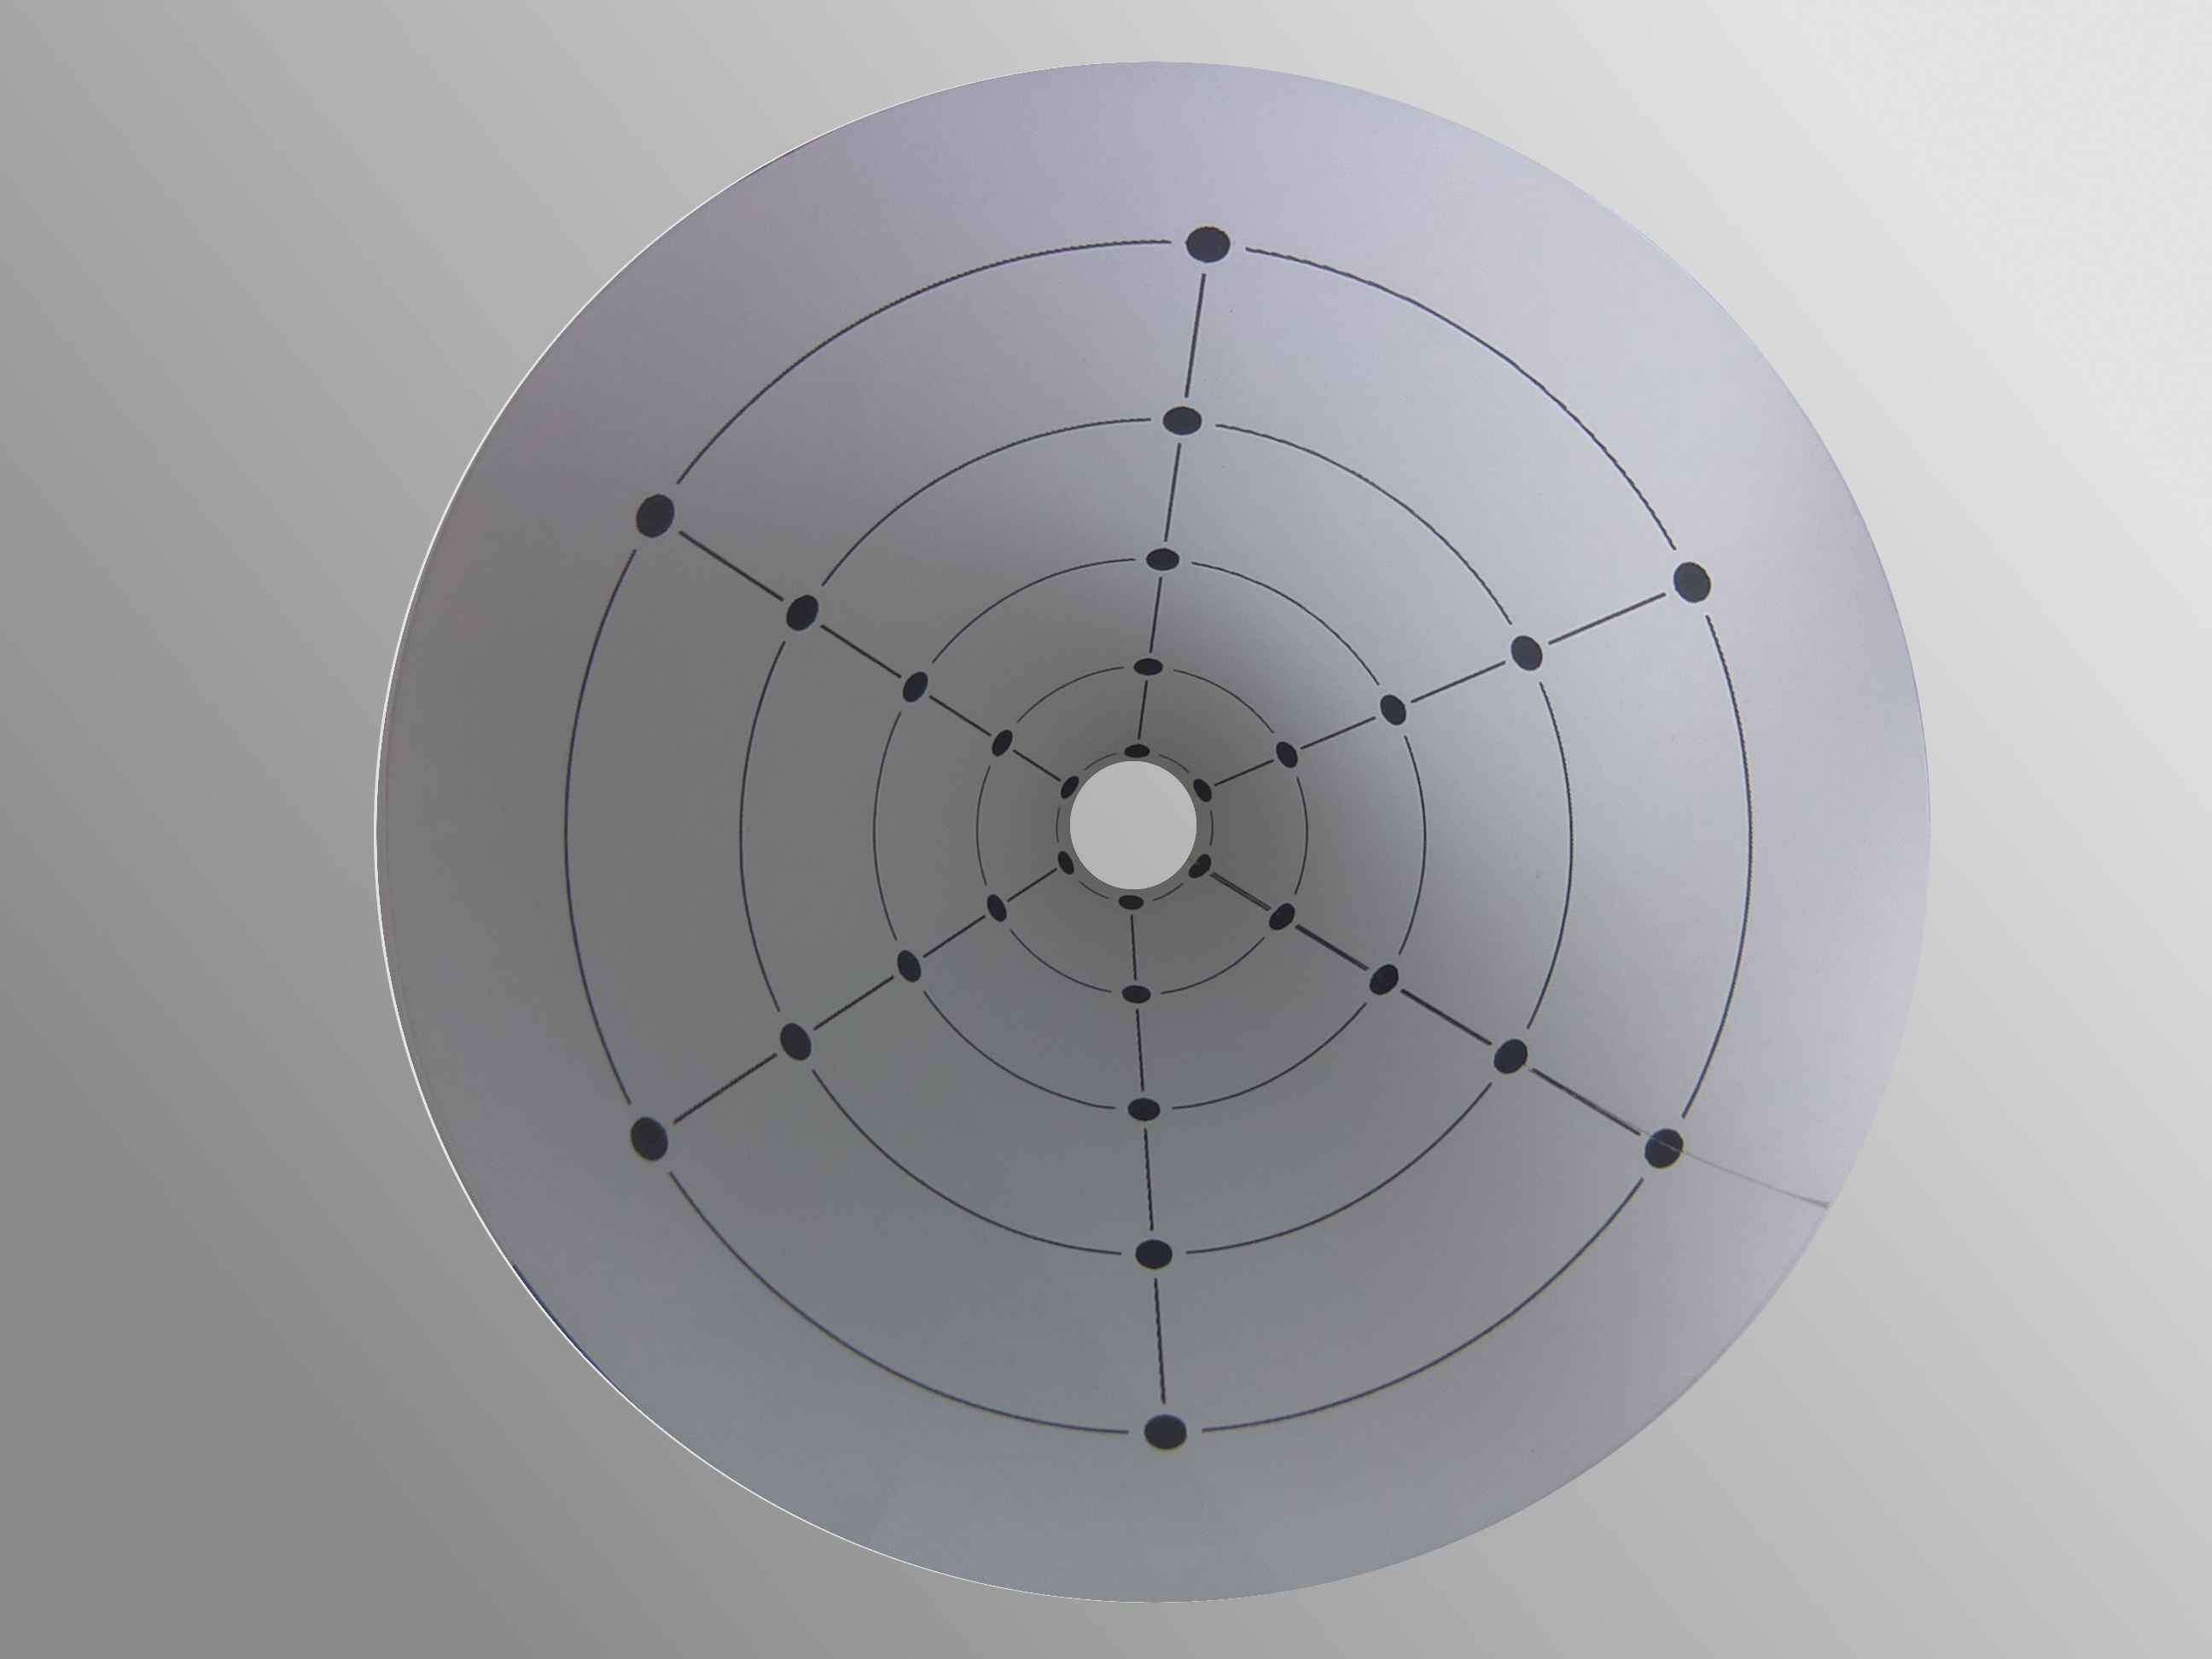
\includegraphics[width=.9\textwidth]{images/coneRasp.jpg}
		\caption{Ursprungsbild}
	\end{subfigure}%
	\begin{subfigure}{.5\textwidth}
		\centering
		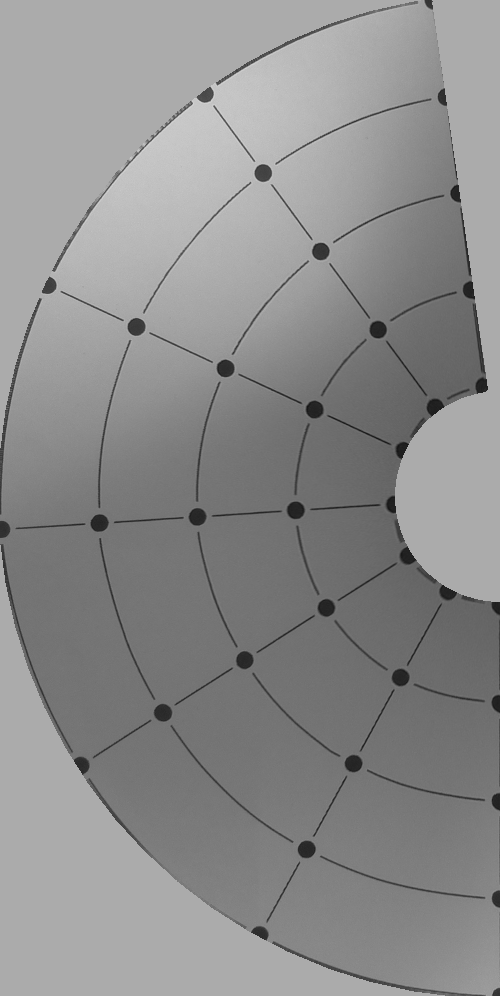
\includegraphics[angle=-90, width=.9\textwidth]{images/coneRaspUnWarpReverse.png}
		\caption{entfaltetes Bild (um 90° im Uhrzeigersinn gedreht)}
	\end{subfigure}
	\caption{Rückwärtsentfaltung}
	\label{fig:reverseUnfold}
\end{figure}
